\documentclass{article}

\usepackage{style}

% Define course name, report name and report title.
\newcommand{\coursename}{Tương tác Người -- Máy (CSC12106)}
\newcommand{\reporttitle}{Hệ thống hỗ trợ đặt lịch, gửi yêu cầu và theo dõi quá trình chăm sóc thú cưng}
% Dùng tiêu đề rút gọn khi \reporttitle dài quá hai dòng trên header.
\newcommand{\headertitle}{Hệ thống hỗ trợ chăm sóc thú cưng}

\newcommand{\studentname}{%
  23127327 -- Lưu Ngô Quốc Bảo\\
  23127328 -- Nguyễn Quốc Bảo\\
  23127498 -- Nguyễn Trọng Tín%
}
\newcommand{\teachername}{%
  Lê Thị Nhàn\\
  Lương Vĩ Minh%
}

% Header
\lhead{\parbox[b]{0.62\textwidth}{%
\setstretch{1}\raggedright\headertitle}}
\rhead{\parbox[b]{0.28\textwidth}{%
\setstretch{1}\raggedleft\coursename}}

% ============ DOCUMENT ============
\begin{document}

\hypersetup{pageanchor=false}
\input{title/title_hcmus}

\hypersetup{pageanchor=true}
\pagenumbering{roman}
\tableofcontents
\pagebreak

\pagenumbering{arabic}

% Main content - 9 chương chuẩn HCI
\section{Giới thiệu}

\subsection{Bối cảnh đề tài}
Trong những năm gần đây, xu hướng nuôi thú cưng tại Việt Nam, đặc biệt ở các đô thị lớn như Thành phố Hồ Chí Minh, đã có bước chuyển dịch mạnh mẽ từ việc nuôi để giữ nhà sang xem thú cưng như những thành viên thân thiết trong gia đình (hiện tượng nhân hóa thú cưng -- pet humanization). Theo các khảo sát thị trường đô thị, nhu cầu sử dụng các dịch vụ chăm sóc thú cưng định kỳ như tắm gội chuyên sâu, vệ sinh tai móng, cắt tỉa tạo kiểu lông (grooming) và dịch vụ trông giữ (pet hotel) ngày càng gia tăng vượt bậc. 

Tuy nhiên, phần lớn các cơ sở dịch vụ thú cưng hiện nay vẫn vận hành dựa trên các phương thức truyền thống mang tính thủ công cao: tiếp nhận đặt lịch qua các cuộc gọi thoại trực tiếp, tin nhắn mạng xã hội (Facebook Fanpage, Zalo cá nhân) hoặc ghi chép tay trên sổ quản lý tiếp nhận tại quầy lễ tân. Trong khi đó, nhóm đối tượng khách hàng chủ đạo sử dụng dịch vụ này lại là những người trẻ, nhân viên văn phòng bận rộn với lịch trình làm việc hành chính dày đặc, ít có thời gian chờ đợi hoặc theo dõi sát sao tại cửa hàng. Sự mất cân đối giữa phương thức tương tác thủ công truyền thống của các cơ sở chăm sóc với thói quen sử dụng công nghệ số tiện lợi, tức thì của chủ nuôi hiện đại đã tạo ra nhiều rào cản và trải nghiệm không mong muốn trong quá trình sử dụng dịch vụ.

Đề tài \textbf{``Hệ thống hỗ trợ đặt lịch, gửi yêu cầu và theo dõi quá trình chăm sóc thú cưng''} được nghiên cứu và phát triển nhằm ứng dụng các nguyên lý Tương tác Người -- Máy (HCI) hiện đại~\cite{Norman2013, Nielsen1994}, số hóa toàn diện quy trình giao tiếp hai chiều giữa chủ nuôi và cơ sở cung cấp dịch vụ, từ đó mang lại trải nghiệm tiện lợi, an tâm và minh bạch tuyệt đối cho người dùng cuối.

\subsection{Phát biểu bài toán}
Thông qua tài liệu Proposal đã được phê duyệt và quá trình khảo sát người dùng thực tế, bài toán cốt lõi mà đồ án tập trung giải quyết xuất phát từ các bất cập nghiêm trọng trong quy trình chăm sóc thú cưng thủ công hiện tại:
\begin{itemize}
    \item \textbf{Khó khăn khi đặt lịch hẹn}: Chủ nuôi phải liên hệ qua điện thoại hoặc nhắn tin nhiều lần để hỏi lịch trống, phải chờ đợi nhân viên rà soát lịch hẹn thủ công. Điều này khiến người dùng rơi vào thế bị động, dễ bị trùng lịch hoặc lỡ mất khung giờ mong muốn trong các dịp cao điểm cuối tuần.
    \item \textbf{Xác nhận thiếu tin cậy và dễ sai lệch}: Việc xác nhận lịch hẹn qua tin nhắn văn bản không đồng bộ tự động vào hệ thống quản lý, dẫn đến rủi ro nhân viên quên ghi sổ hoặc ghi nhận nhầm lẫn thông tin thời gian, loại dịch vụ và nhân sự phụ trách.
    \item \textbf{Thất lạc dặn dò y tế và yêu cầu đặc biệt}: Thú cưng thường có tiền sử sức khỏe riêng biệt (như dị ứng với một số thành phần xà phòng thơm, bệnh da liễu nhạy cảm, vừa phẫu thuật cần tránh nước, hoặc tính cách hoảng sợ khi sấy lông). Trong quy trình cũ, chủ nuôi phải liên tục nhắc đi nhắc lại các lưu ý này mỗi khi gửi thú cưng. Nhân viên tiếp nhận tại quầy ghi chép sơ sài hoặc không bàn giao đầy đủ cho kỹ thuật viên trực tiếp tắm cắt, dẫn đến tai nạn tái phát dị ứng nguy hiểm hoặc thú cưng bị hoảng loạn.
    \item \textbf{Thiếu cập nhật tiến độ theo thời gian thực}: Trong suốt khoảng thời gian 2--3 giờ thú cưng được gửi tại cơ sở, chủ nuôi hoàn toàn không nắm bắt được thú cưng của mình đang ở giai đoạn nào (đã được tắm chưa, đang cắt tỉa hay đã xong). Trạng thái ``mù mờ'' thông tin này gây nên tâm lý bất an, lo lắng cho chủ nuôi nhưng họ lại ngại gọi điện làm phiền nhân viên đang bận tay thao tác.
    \item \textbf{Thiếu lịch sử chăm sóc có cấu trúc}: Toàn bộ dữ liệu về các lần sử dụng dịch vụ trước (loại dầu tắm đã dùng có hợp da hay không, độ dài cắt tỉa phù hợp, tình trạng da lông phát hiện lúc tắm, chi phí dịch vụ) đều bị trôi mất trong các chuỗi tin nhắn trò chuyện rời rạc, gây khó khăn cho việc theo dõi sức khỏe lâu dài của thú cưng.
\end{itemize}

Hệ quả là cả chủ nuôi lẫn cơ sở chăm sóc đều lãng phí nhiều thời gian liên lạc lặp đi lặp lại, gia tăng nguy cơ sai sót y tế và làm suy giảm sự gắn kết tin cậy giữa hai bên.

\subsection{Mục tiêu đề tài}
Đồ án hướng tới các mục tiêu cụ thể, bám sát định hướng giải pháp đã cam kết trong Proposal:
\begin{itemize}
    \item \textbf{Mục tiêu tương tác \& Trải nghiệm người dùng (UX/Usability Goals)}:
    \begin{enumerate}
        \item \textit{Tính hiệu quả (Effectiveness)}: Đảm bảo chủ nuôi đặt lịch chính xác 100\% vào các khung giờ trống thực tế và thông tin dặn dò y tế được chuyển giao nguyên vẹn tới kỹ thuật viên phụ trách.
        \item \textit{Hiệu suất (Efficiency)}: Rút ngắn thời gian thao tác đặt lịch xuống dưới 1 phút; cung cấp khả năng tra cứu tiến độ và lịch sử chỉ với 1--2 thao tác chạm trên thiết bị di động.
        \item \textit{Phòng ngừa sai sót (Error Prevention)}: Tự động khóa các khung giờ đã kín; thiết kế cơ chế cảnh báo thị giác nổi bật (visual alert) đối với các trường hợp dị ứng hoặc chống chỉ định y tế.
        \item \textit{Sự an tâm \& Hài lòng (Satisfaction \& Peace of Mind)}: Xóa bỏ hoàn toàn trạng thái lo âu của chủ nuôi khi gửi thú cưng bằng hệ thống cập nhật 4 mốc thời gian thực minh bạch.
    \end{enumerate}
    \item \textbf{Mục tiêu sản phẩm thiết kế}:
    \begin{enumerate}
        \item Xây dựng hoàn chỉnh kiến trúc thông tin, luồng tác vụ và bộ khung giao diện Wireframe chuẩn Mobile-first.
        \item Thiết kế bản mẫu tương tác độ nét cao (High-fidelity Interactive Prototype) trên Figma thể hiện trọn vẹn 4 mục tiêu cốt lõi của Persona chính (Persona 1).
        \item Đánh giá tính khả dụng thực tế thông qua các chỉ số định lượng (Task Completion Rate, Time on Task, Error Rate, Điểm khảo sát Likert/SUS) để làm cơ sở tinh chỉnh thiết kế cuối cùng.
    \end{enumerate}
\end{itemize}

\subsection{Phạm vi đề tài}
\begin{itemize}
    \item \textbf{Phạm vi thực hiện (In-Scope)}:
    \begin{itemize}
        \item Tập trung toàn diện vào trải nghiệm giao diện người dùng của \textbf{Chủ nuôi thú cưng (Pet Owners)} trên nền tảng Web di động (Mobile Web).
        \item Triển khai trọn vẹn \textbf{4 trụ cột chức năng cốt lõi}:
        \begin{enumerate}
            \item \textit{Đặt lịch có xác nhận tức thì}: Chọn thú cưng, chọn gói dịch vụ, duyệt khung giờ trống và nhận thông báo xác nhận tự động.
            \item \textit{Hồ sơ thú cưng \& Dặn dò đặc biệt}: Quản lý thông tin sức khỏe, lưu ý dị ứng/thuốc và tự động đồng bộ vào đơn tiếp nhận dịch vụ kèm mã QR Check-in.
            \item \textit{Theo dõi tiến độ thời gian thực (Live Tracking)}: Thanh tiến trình hiển thị minh bạch 4 mốc trạng thái chuẩn (\textit{Đã nhận thú cưng} $\rightarrow$ \textit{Đang chăm sóc} $\rightarrow$ \textit{Hoàn tất} $\rightarrow$ \textit{Chờ đón}) kết hợp thông báo đẩy (Push Notification).
            \item \textit{Lịch sử chăm sóc cá nhân hóa}: Lưu trữ nhật ký từng buổi dịch vụ, tên sản phẩm chuyên dụng đã sử dụng, ghi chú kỹ thuật viên và hóa đơn điện tử minh bạch.
        \end{enumerate}
    \end{itemize}
    \item \textbf{Phạm vi không thực hiện (Out-of-Scope)}:
    \begin{itemize}
        \item Không xây dựng toàn bộ hệ thống quản trị nội bộ ERP phức tạp cho chuỗi cửa hàng (quản lý kho bãi lớn, quản lý chấm công, tính lương nhân sự).
        \item Không tích hợp luồng phát trực tiếp camera giám sát vật lý tại chuồng do giới hạn bảo mật và băng thông hạ tầng mạng trong phạm vi đồ án môn học.
    \end{itemize}
\end{itemize}

\section{Nghiên cứu người dùng}

\subsection{Đối tượng người dùng mục tiêu}
Đối tượng người dùng mục tiêu của hệ thống là những chủ nuôi thú cưng (Pet Owners) đang sinh sống và làm việc tại các đô thị lớn (tiêu biểu là TP. Hồ Chí Minh). Họ là những người trực tiếp lựa chọn gói dịch vụ, thực hiện đặt lịch, khai báo yêu cầu chăm sóc, đưa đón và theo dõi tình trạng thú cưng.

Đặc điểm nhân khẩu học và hành vi nổi bật của nhóm đối tượng này bao gồm:
\begin{itemize}
    \item \textbf{Độ tuổi}: Từ 20 đến 35 tuổi (chủ yếu là sinh viên đại học, nhân viên văn phòng, chuyên viên phân tích, người làm việc tự do).
    \item \textbf{Mức độ am hiểu công nghệ}: Cao; có thói quen sử dụng điện thoại thông minh hàng ngày cho các tác vụ thương mại điện tử, đặt dịch vụ và thanh toán không tiền mặt.
    \item \textbf{Lối sống và quỹ thời gian}: Bận rộn với lịch học tập và làm việc dày đặc, không có nhiều thời gian rảnh để gọi điện trao đổi dài dòng hoặc ngồi chờ trực tiếp tại cơ sở spa.
    \item \textbf{Tâm lý và kỳ vọng}: Coi thú cưng như con cái hoặc thành viên ruột thịt; rất quan tâm đến sức khỏe, sự an toàn và tính thoải mái của thú cưng, nhưng luôn có tâm lý e ngại việc dặn dò đặc biệt (về bệnh ngoài da, dị ứng hoặc tính cách nhút nhát) bị nhân viên bỏ quên.
\end{itemize}

\subsection{Phương pháp nghiên cứu}
Để thu thập dữ liệu chân thực và sâu sắc về hành vi và khó khăn của người dùng, nhóm đã áp dụng kết hợp hai phương pháp nghiên cứu định tính và định lượng chuẩn HCI:
\begin{enumerate}
    \item \textbf{Phỏng vấn sâu theo ngữ cảnh (Contextual In-depth Interview)}: Thực hiện phỏng vấn trực tiếp và bán cấu trúc với 6 chủ nuôi thú cưng có hồ sơ đa dạng (từ chủ nuôi có thú cưng bị dị ứng mạn tính đến sinh viên nuôi mèo nhút nhát). Mục đích nhằm đào sâu vào cảm xúc, trải nghiệm thực tế trong các lần đưa thú cưng đi spa trước đây, cũng như nguyên nhân sâu xa của sự bất an khi giao thú cưng cho tiệm.
    \item \textbf{Khảo sát bằng bảng câu hỏi trực tuyến (Online Survey)}: Thu thập ý kiến phản hồi về tần suất chăm sóc thú cưng, mức độ hài lòng với các kênh liên lạc truyền thống (gọi điện thoại, nhắn tin Fanpage/Zalo) và các tính năng mong đợi nhất trên một ứng dụng chuyên biệt.
\end{enumerate}

\subsection{Kết quả nghiên cứu}
Từ các dữ liệu phỏng vấn và khảo sát thực tế tại thư mục dữ liệu nghiên cứu (\texttt{data/user-research/}), nhóm đã tổng hợp được các phát hiện then chốt sau:
\begin{itemize}
    \item \textbf{Về thời gian đặt lịch}: $83.3\%$ người tham gia cho biết họ cảm thấy phiền phức khi phải nhắn tin hỏi giờ trống và chờ cơ sở phản hồi; $50\%$ từng gặp sự cố bị trùng lịch hoặc đến nơi nhưng tiệm quá đông phải chờ đợi hàng giờ.
    \item \textbf{Về ghi nhớ thông tin dị ứng \& an toàn y tế}: $100\%$ chủ nuôi có thú cưng bị dị ứng da hoặc có tính cách đặc biệt bày tỏ sự bức xúc vì lần nào gửi cũng phải dặn đi dặn lại nhân viên. Đã có trường hợp thú cưng bị tái phát viêm da nặng hoặc trầy xước do tiệm sơ suất dùng sai dầu tắm hoặc nhốt chung với thú cưng hung dữ.
    \item \textbf{Về nhu cầu theo dõi tiến độ}: $100\%$ người dùng thừa nhận họ có cảm giác bất an, lo lắng trong suốt thời gian thú cưng ở tiệm. Họ muốn biết rõ thú cưng đang làm đến bước nào mà không cần phải gọi điện làm phiền nhân viên.
    \item \textbf{Về quản lý lịch sử dịch vụ}: Đa số người dùng không thể nhớ chính xác lần trước mình đã dùng loại sữa tắm nào, dịch vụ cắt tỉa gì hay chi phí bao nhiêu do thông tin bị phân tán trong các tin nhắn chat cũ.
\end{itemize}

\subsection{Nhu cầu và điểm đau của người dùng}
Tổng hợp từ kết quả nghiên cứu, nhóm đã xác định 4 nhóm nhu cầu cốt lõi đối ứng trực tiếp với 4 điểm đau lớn của người dùng:
\begin{table}[H]
\centering
\begin{tabularx}{\textwidth}{|l|X|X|}
\hline
\textbf{STT} & \textbf{Điểm đau của người dùng} & \textbf{Nhu cầu tương ứng của người dùng} \\ \hline
1 & Chờ đợi lâu khi hỏi lịch, xác nhận thủ công dễ bị sót hoặc nhầm lẫn thời gian. & Xem trực tiếp ma trận khung giờ còn trống và nhận xác nhận lịch hẹn tức thì trên ứng dụng. \\ \hline
2 & Thất lạc dặn dò đặc biệt về tiền sử dị ứng xà phòng, bệnh ngoài da, thuốc và tính cách. & Hồ sơ thú cưng điện tử lưu vĩnh viễn cảnh báo y tế và tự động gắn vào phiếu tiếp nhận của kỹ thuật viên. \\ \hline
3 & Bất an suốt 2--3 tiếng chăm sóc, không biết tình trạng thú cưng, ngại gọi điện hỏi. & Theo dõi tiến độ thời gian thực qua 4 mốc rõ ràng và nhận thông báo đẩy khi chuyển giai đoạn. \\ \hline
4 & Thông tin chi phí, loại dịch vụ và sản phẩm đã dùng bị trôi tin, không thể tra cứu lại. & Kho lưu trữ lịch sử chăm sóc cá nhân hóa, hiển thị chi tiết hóa đơn điện tử và phác đồ đã sử dụng. \\ \hline
\end{tabularx}
\caption{Tổng hợp điểm đau và nhu cầu cốt lõi của người dùng}
\label{tab:pains_needs}
\end{table}

\subsection{Chân dung người dùng}
Dựa trên kết quả nghiên cứu định tính và định lượng, nhóm xây dựng hai Persona đại diện hoàn chỉnh cho hai phân khúc người dùng mục tiêu của hệ thống:

\subsubsection{Chân dung người dùng 1: Nguyễn Hoàng Lan}
\begin{itemize}
    \item \textbf{Vai trò}: Chân dung người dùng chính (Primary Persona).
    \item \textbf{Thông tin cá nhân}: 28 tuổi, Nữ, Chuyên viên Phân tích Dữ liệu (Data Analyst) tại Quận 1, TP.HCM; thu nhập 22.000.000 VNĐ/tháng.
    \item \textbf{Thông tin thú cưng}: Chó Poodle 2 tuổi (tên Bơ, 4.5kg). Bơ có tiền sử viêm da dị ứng với xà phòng nhiều hương liệu và nhút nhát với tiếng máy sấy công suất lớn.
    \item \textbf{Trích dẫn}: \textit{''Mình rất bận nên chỉ mong đặt lịch nhanh có xác nhận ngay, gửi bé đi tắm có thể theo dõi tiến độ từ xa và tiệm luôn nhớ bé bị dị ứng da để chăm sóc an toàn.''}
    \item \textbf{Mục tiêu cốt lõi}:
    \begin{enumerate}
        \item Đặt lịch dịch vụ chăm sóc nhanh chóng, có xác nhận tức thì mà không cần chờ đợi.
        \item Đảm bảo tiệm tiếp nhận và thực hiện đúng lưu ý đặc biệt về tiền sử dị ứng xà phòng của Bơ.
        \item Theo dõi tiến độ 4 mốc thời gian thực để chủ động thời gian đón bé mà không cần gọi điện.
        \item Lưu trữ và tra cứu lịch sử các lần chăm sóc trước (sản phẩm, chi phí, ghi chú kỹ thuật viên).
    \end{enumerate}
    \item \textbf{Điểm đau chính}: Phải gọi điện/nhắn tin hỏi lịch; lần nào cũng phải nhắc lại tiền sử dị ứng; lo lắng suốt 2--3 tiếng làm dịch vụ; thông tin cũ bị thất lạc trong tin nhắn.
    \item \textbf{Bằng chứng truy vết}: \texttt{deliverables/01-user-research/persona/personas.json}, \texttt{data/user-research/06\_interview\_member.md}, \texttt{docs/proposal.md}.
\end{itemize}

\begin{figure}[H]
\centering

\includegraphics[height=0.60\textheight, keepaspectratio]{persona-1.png}
\caption{Chân dung người dùng chính -- Nguyễn Hoàng Lan (Primary Persona)}
\label{fig:persona_1}
\end{figure}

\subsubsection{Chân dung người dùng 2: Trần Minh Khoa}
\begin{itemize}
    \item \textbf{Vai trò}: Chân dung người dùng phụ (Secondary Persona).
    \item \textbf{Thông tin cá nhân}: 21 tuổi, Nam, Sinh viên Đại học năm 3 tại TP. Thủ Đức, TP.HCM; thu nhập 5.000.000 VNĐ/tháng.
    \item \textbf{Thông tin thú cưng}: Mèo Anh lông ngắn 1.5 tuổi (tên Miu, 3.8kg). Miu rất nhút nhát, sợ tiếng ồn lớn và người lạ, dễ hoảng loạn nếu gặp thú dữ. Từng bị sự cố trầy xước do tiệm cũ nhốt chung buồng.
    \item \textbf{Trích dẫn}: \textit{''Mèo của mình rất nhút nhát nên mình rất sợ gửi tiệm bị nhốt chung với bé dữ. Mình chỉ muốn biết rõ tiến độ chăm sóc và có hồ sơ lưu lại dặn dò để tiệm không quên.''}
    \item \textbf{Mục tiêu cốt lõi}:
    \begin{enumerate}
        \item Biết trước khung giờ vắng khách để đặt lịch, tránh cho mèo bị hoảng loạn.
        \item Nắm bắt được tình trạng của mèo từ xa trong suốt quá trình làm dịch vụ để an tâm tuyệt đối.
        \item Tra cứu lại chi phí, loại dịch vụ và lịch sử các lần chăm sóc để quản lý ngân sách sinh viên.
    \end{enumerate}
    \item \textbf{Điểm đau chính}: Đến tiệm mới biết hết chỗ; ám ảnh sự cố thú cưng bị tổn thương do bất cẩn; ngại gọi điện thoại làm phiền; không có nơi lưu trữ hóa đơn rõ ràng.
    \item \textbf{Bằng chứng truy vết}: \texttt{deliverables/01-user-research/persona/personas.json}, \texttt{data/user-research/01\_respondent\_08-06.md}, \texttt{data/user-research/02\_respondent\_08-07\_0503.md}.
\end{itemize}

\begin{figure}[H]
\centering

\includegraphics[height=0.60\textheight, keepaspectratio]{persona-2.png}
\caption{Chân dung người dùng phụ -- Trần Minh Khoa (Secondary Persona)}
\label{fig:persona_2}
\end{figure}

\subsection{Đề xuất giá trị}
Tương ứng với hai Persona đại diện, nhóm đã thiết lập hai bản Đề xuất giá trị (Value Proposition Canvas) theo mô hình chuẩn của Osterwalder et al.\cite{osterwalder2014value}, thể hiện sự khớp nối 1--1 hoàn hảo giữa Hồ sơ khách hàng (Customer Profile) và Bản đồ giá trị (Value Map):

\subsubsection{Đề xuất giá trị đối ứng cho Persona 1: Nguyễn Hoàng Lan}
\begin{itemize}
    \item \textbf{Hồ sơ khách hàng (Customer Profile)}:
    \begin{itemize}
        \item \textit{Tác vụ của khách hàng (Customer Jobs)}: Đặt lịch spa/cắt tỉa định kỳ nhanh chóng (J1); Dặn dò chi tiết tiền sử dị ứng xà phòng và tính nhút nhát của Poodle Bơ (J2); Theo dõi trạng thái chăm sóc từ xa trong giờ làm việc (J3); Tra cứu lại nhật ký dịch vụ và sản phẩm sử dụng trước đây (J4).
        \item \textit{Điểm đau (Pains)}: Chờ đợi lâu khi hỏi lịch (P1); Tiệm quên dặn dò dị ứng gây tái phát bệnh ngoài da (P2 - Mức độ nghiêm trọng); Bất an không biết tiến độ của bé đến đâu (P3); Lịch sử chăm sóc bị thất lạc trong tin nhắn chat (P4).
        \item \textit{Yếu tố tạo lợi ích mong đợi (Gains)}: Xem lịch trống và xác nhận tức thì (G1); An tâm tuyệt đối khi dặn dò dị ứng được hiển thị rõ ràng trên phiếu tiếp nhận (G2); Nhận thông báo chủ động theo 4 mốc thời gian thực (G3); Hồ sơ số hóa tập trung, tra cứu nhanh chỉ với một chạm (G4).
    \end{itemize}
    \item \textbf{Bản đồ giá trị (Value Map)}:
    \begin{itemize}
        \item \textit{Sản phẩm và Dịch vụ (Products \& Services)}: Đặt lịch trực tuyến với ma trận giờ trống thời gian thực (S1); Hồ sơ thú cưng tự động gắn cảnh báo dị ứng y tế (S2); Bảng theo dõi tiến độ 4 mốc kèm thông báo đẩy (S3); Kho lưu trữ lịch sử chăm sóc cá nhân hóa (S4).
        \item \textit{Trợ thủ giải tỏa đau đớn (Pain Relievers)}: Khóa giữ chỗ và xác nhận lịch tức thì, xóa bỏ thời gian chờ phản hồi (PR1); Gắn nhãn dị ứng nổi bật vào phiếu bàn giao ca, triệt tiêu rủi ro bỏ sót dặn dò (PR2); Cập nhật tiến độ tự động qua thông báo đẩy, xóa tan bất an (PR3); Tự động lưu trữ chi tiết dịch vụ và loại sữa tắm sau mỗi lượt (PR4).
        \item \textit{Yếu tố tạo lợi ích (Gain Creators)}: Tiết kiệm tối đa thời gian đặt lịch (GC1); Đảm bảo quy trình chăm sóc an toàn chuẩn y tế cho da nhạy cảm (GC2); Chủ động 100\% thời gian cá nhân nhờ thông báo khi chuyển mốc Chờ đón (GC3); Dễ dàng theo dõi sức khỏe dài hạn (GC4).
    \end{itemize}
\end{itemize}

\begin{figure}[H]
\centering

\includegraphics[width=0.90\textwidth, keepaspectratio]{value-proposition-1.png}
\caption{Bản đề xuất giá trị đối ứng cho Persona 1 -- Nguyễn Hoàng Lan}
\label{fig:vp_1}
\end{figure}

\subsubsection{Đề xuất giá trị đối ứng cho Persona 2: Trần Minh Khoa}
\begin{itemize}
    \item \textbf{Hồ sơ khách hàng (Customer Profile)}:
    \begin{itemize}
        \item \textit{Tác vụ của khách hàng (Customer Jobs)}: Tìm và đặt lịch vào khung giờ vắng khách để tránh mèo bị hoảng loạn (J1); Nắm bắt trạng thái từ xa để kịp thời đến đón ngay khi hoàn tất (J2); Kiểm tra bảng giá minh bạch và lưu lại hóa đơn chi tiết (J3).
        \item \textit{Điểm đau (Pains)}: Đến tiệm mới biết đông khách hoặc hết chỗ (P1); Rất lo lắng cho mèo nhút nhát nhưng ngại gọi điện thoại (P2); Không có nơi lưu trữ hóa đơn, khó quản lý chi tiêu (P3).
        \item \textit{Yếu tố tạo lợi ích mong đợi (Gains)}: Chủ động chọn khung giờ thưa khách và nhận xác nhận lịch trước (G1); Cập nhật tiến độ theo từng mốc để đón mèo sớm nhất (G2); Minh bạch toàn bộ chi phí và lưu trữ hóa đơn điện tử (G3).
    \end{itemize}
    \item \textbf{Bản đồ giá trị (Value Map)}:
    \begin{itemize}
        \item \textit{Sản phẩm và Dịch vụ (Products \& Services)}: Hiển thị khung giờ trống và mật độ khách, hỗ trợ đặt lịch giữ chỗ tức thì (S1); Trình hiển thị tiến độ 4 mốc chuẩn xác và thông báo đẩy khi hoàn tất (S2); Sổ theo dõi lịch sử dịch vụ tích hợp bảng giá và hóa đơn điện tử (S3).
        \item \textit{Trợ thủ giải tỏa đau đớn (Pain Relievers)}: Loại bỏ hoàn toàn tình trạng chờ đợi tại chỗ (PR1); Xóa tan sự e ngại gọi điện nhờ cơ chế tự động gửi thông báo theo mốc (PR2); Minh bạch 100\% giá dịch vụ và lưu trữ đầy đủ hóa đơn (PR3).
        \item \textit{Yếu tố tạo lợi ích (Gain Creators)}: Giúp chủ nuôi chủ động chọn thời điểm yên tĩnh nhất cho thú cưng nhút nhát (GC1); Tối ưu thời gian đón ngay khi có thông báo Chờ đón (GC2); Dễ dàng đối soát chi phí và quản lý ngân sách nuôi thú cưng (GC3).
    \end{itemize}
\end{itemize}

\begin{figure}[H]
\centering

\includegraphics[width=0.90\textwidth, keepaspectratio]{value-proposition-2.png}
\caption{Bản đề xuất giá trị đối ứng cho Persona 2 -- Trần Minh Khoa}
\label{fig:vp_2}
\end{figure}

\section{Yêu cầu và mục tiêu thiết kế}

\subsection{Yêu cầu người dùng}
Dựa trên kết quả nghiên cứu và Đề xuất giá trị ở Chương 2, các nhu cầu và điểm đau của người dùng được chuyển hóa thành 4 nhóm \textbf{Yêu cầu người dùng (User Requirements -- UR)} cốt lõi, bám sát 4 trụ cột giải pháp trong tài liệu đề xuất đề tài:

\begin{enumerate}
    \item \textbf{UR1 -- Đặt lịch trực tuyến và nhận xác nhận tức thì (Instant Booking Confirmation)}:
    \begin{itemize}
        \item Người dùng có thể xem danh sách dịch vụ kèm bảng giá công khai, thời lượng dự kiến và danh sách các khung giờ còn trống trong ngày/tuần.
        \item Hệ thống phải tự động khóa các khung giờ đã kín chỗ, chỉ cho phép chọn các khung giờ khả dụng.
        \item Sau khi xác nhận thông tin, hệ thống phải cấp mã đặt lịch và xác nhận giữ chỗ ngay lập tức trên ứng dụng, không bắt người dùng phải chờ nhân viên phản hồi thủ công.
    \end{itemize}
    \item \textbf{UR2 -- Hồ sơ thú cưng điện tử và tự động đính kèm cảnh báo y tế (Medical Profile \& Auto-attachment)}:
    \begin{itemize}
        \item Cho phép tạo và quản lý hồ sơ cho nhiều thú cưng (chó, mèo), lưu trữ giống loài, cân nặng, tiền sử viêm da dị ứng xà phòng, dặn dò tính cách (nhút nhát, sợ máy sấy, yêu cầu phòng cách ly).
        \item Khi người dùng đặt lịch cho một thú cưng cụ thể, hệ thống phải tự động liên kết các cảnh báo y tế và dặn dò đặc biệt từ hồ sơ vào đơn tiếp nhận dịch vụ.
        \item Thẻ cảnh báo y tế phải được làm nổi bật với màu sắc và biểu tượng tương phản cao trên phiếu bàn giao ca của cơ sở.
    \end{itemize}
    \item \textbf{UR3 -- Theo dõi tiến độ chăm sóc theo thời gian thực (Real-time Live Tracking)}:
    \begin{itemize}
        \item Cung cấp giao diện thanh tiến trình thời gian thực chuẩn hóa qua 4 mốc: \textbf{Mốc 1 (Đã nhận thú cưng)} $\rightarrow$ \textbf{Mốc 2 (Đang chăm sóc)} $\rightarrow$ \textbf{Mốc 3 (Hoàn tất dịch vụ)} $\rightarrow$ \textbf{Mốc 4 (Sẵn sàng chờ đón)}.
        \item Mỗi mốc hiển thị thời gian ghi nhận thực tế và thời gian hoàn tất dự kiến; hỗ trợ gửi thông báo đẩy tự động khi trạng thái chuyển mốc.
        \item Cho phép chủ nuôi xem hình ảnh kiểm tra sức khỏe sơ bộ tại tiệm và gửi dặn dò bổ sung trực tiếp cho kỹ thuật viên trong suốt ca chăm sóc.
    \end{itemize}
    \item \textbf{UR4 -- Kho lưu trữ lịch sử chăm sóc cá nhân hóa và hóa đơn điện tử (Care History \& Digital Invoice)}:
    \begin{itemize}
        \item Lưu trữ toàn bộ nhật ký các lượt chăm sóc theo dòng thời gian, bao gồm ngày giờ, gói dịch vụ, loại sản phẩm sữa tắm trị liệu đã dùng và ghi chú của kỹ thuật viên.
        \item Cung cấp hóa đơn điện tử minh bạch từng hạng mục chi phí và biểu đồ theo dõi ngân sách chi tiêu hàng tháng.
        \item Cho phép đặt lại nhanh (\textit{One-click Rebook}) dựa trên thông tin gói dịch vụ của lượt chăm sóc trước.
    \end{itemize}
\end{enumerate}

Bảng \ref{tab:traceability_ur} thể hiện ma trận truy vết từ Phát hiện nghiên cứu $\rightarrow$ Điểm đau $\rightarrow$ Yêu cầu người dùng tương ứng.

\begin{table}[H]
\centering
\small
\begin{tabularx}{\textwidth}{|l|X|X|l|}
\hline
\textbf{Mã UR} & \textbf{Nguồn phát hiện nghiên cứu} & \textbf{Điểm đau giải quyết} & \textbf{Trụ cột đề tài} \\ \hline
\textbf{UR1} & 100\% người dùng phàn nàn về việc chờ phản hồi tin nhắn đặt lịch (15--120 phút). & Chờ đợi lâu, dễ bị trùng lịch hoặc lỡ khung giờ mong muốn. & Đặt lịch tức thì \\ \hline
\textbf{UR2} & 83.3\% chủ nuôi có thú cưng da nhạy cảm lo ngại tiệm quên dặn dò khi đổi ca trực. & Thất lạc lưu ý y tế, nguy cơ tái phát dị ứng da hoặc hoảng loạn. & Hồ sơ dặn dò y tế \\ \hline
\textbf{UR3} & 90\% chủ nuôi bất an trong 2--3 tiếng chăm sóc nhưng ngại gọi điện làm phiền. & Trạng thái mù mờ thông tin, gián đoạn công việc hai bên. & Theo dõi 4 mốc \\ \hline
\textbf{UR4} & 100\% người dùng không có công cụ lưu trữ lịch sử dịch vụ và đối soát chi phí. & Thất lạc hóa đơn, không nhớ loại dầu tắm cũ, khó quản lý chi tiêu. & Lịch sử cá nhân hóa \\ \hline
\end{tabularx}
\caption{Ma trận truy vết Yêu cầu người dùng từ dữ liệu nghiên cứu}
\label{tab:traceability_ur}
\end{table}

\subsection{Mục tiêu trải nghiệm người dùng}
Để đo lường chất lượng tương tác và tính khả dụng của giải pháp thiết kế, nhóm đã xác định 6 \textbf{Mục tiêu trải nghiệm người dùng (UX Goals)} dựa trên các nguyên lý chuẩn mực của Nielsen và Norman \cite{nielsen1994usability, norman2013design}:

\begin{itemize}
    \item \textbf{Tính hiệu quả (Effectiveness)}: Đảm bảo người dùng hoàn thành chính xác 100\% các tác vụ cốt lõi (đặt lịch, lưu dặn dò dị ứng, theo dõi tiến độ, tra cứu lịch sử) mà không gặp phải sự cố tắc nghẽn giao diện.
    \item \textbf{Hiệu suất thao tác (Efficiency)}: Tối ưu hóa số bước thao tác và độ trễ nhận thức; đặt mục tiêu hoàn thành toàn bộ luồng đặt lịch trong vòng dưới 45 giây và xem trạng thái chăm sóc chỉ trong 1 lần chạm (dưới 20 giây).
    \item \textbf{Tính dễ học (Learnability)}: Giao diện tuân thủ các mô hình tinh thần (\textit{mental models}) quen thuộc của ứng dụng di động hiện đại, giúp người dùng mới nắm bắt quy trình ngay từ lần đầu tiên mà không cần đọc tài liệu hướng dẫn.
    \item \textbf{Phòng ngừa sai sót (Error Prevention)}: Thiết kế hệ thống phòng vệ chủ động: tự động vô hiệu hóa các khung giờ đã kín, cảnh báo xung đột gói dịch vụ với tiền sử dị ứng và xác nhận lại thông tin trước khi gửi đơn.
    \item \textbf{Sự an tâm và hài lòng (Emotional Peace of Mind \& Satisfaction)}: Giải tỏa căng thẳng tâm lý cho chủ nuôi bằng cách cung cấp thông tin minh bạch theo thời gian thực; điểm đánh giá SUS đạt trên 80/100 điểm.
    \item \textbf{Khả năng ghi nhớ (Memorability)}: Bố cục trực quan và quy trình chuẩn hóa giúp người dùng có thể thực hiện lại các tác vụ định kỳ một cách tự nhiên sau thời gian dài không sử dụng.
\end{itemize}

\subsection{Mục tiêu thiết kế}
Từ các yêu cầu và mục tiêu trải nghiệm, nhóm đã cụ thể hóa thành 4 \textbf{Mục tiêu thiết kế (Design Goals -- DG)} định hướng trực tiếp cho việc xây dựng Wireframe và Prototype:

\begin{enumerate}
    \item \textbf{DG1 -- Thiết kế luồng đặt lịch trực quan dạng từng bước (Stepper Flow)}: Phân tách rõ ràng các bước: Chọn thú cưng $\rightarrow$ Chọn gói dịch vụ $\rightarrow$ Chọn ngày và ma trận giờ trống $\rightarrow$ Xác nhận tóm tắt. Sử dụng các thẻ bấm lớn (\textit{touch targets} $\ge 44 \times 44\text{px}$), phản hồi thị giác tức thì khi chọn khung giờ.
    \item \textbf{DG2 -- Thiết kế hệ thống cảnh báo y tế nổi bật với độ tương phản cao}: Sử dụng các thành phần giao diện chuyên biệt (Badge màu đỏ \texttt{\#DC2626} cho dị ứng, màu vàng cam \texttt{\#D97706} cho lưu ý hành vi), luôn hiển thị đồng bộ từ màn hình Hồ sơ, Form đặt lịch cho đến Phiếu tiếp nhận QR và màn hình bàn giao ca.
    \item \textbf{DG3 -- Thiết kế thanh tiến trình 4 mốc thời gian thực trực quan}: Xây dựng thành phần \textit{Timeline Stepper} 4 mốc với biểu tượng rõ ràng, phân biệt rành mạch giữa các trạng thái \textit{Đã hoàn thành} (Xanh lá \texttt{\#16A34A}), \textit{Đang diễn ra} (Xanh dương \texttt{\#173B72} có hiệu ứng nhịp thở) và \textit{Chưa đến} (Xám mờ \texttt{\#9CA3AF}).
    \item \textbf{DG4 -- Thiết kế trung tâm quản lý lịch sử và chi phí thông minh}: Cung cấp thẻ tóm tắt chi phí, bộ lọc thông minh theo tháng/thú cưng, hiển thị chi tiết sản phẩm đã dùng kèm nút ``Đặt lại ngay'' giúp tái sử dụng thông tin cũ chỉ với một chạm.
\end{enumerate}

\section{Phân tích hệ thống và trải nghiệm hiện tại}

\subsection{Hệ thống và quy trình hiện tại}
Hiện nay, hầu hết các cơ sở spa và chăm sóc thú cưng quy mô vừa và nhỏ tại Việt Nam chưa áp dụng hệ thống phần mềm chuyên biệt phục vụ trải nghiệm của khách hàng. Quy trình tương tác giữa chủ nuôi và cơ sở chủ yếu diễn ra qua ba kênh phân mảnh:
\begin{itemize}
    \item \textbf{Kênh gọi điện thoại trực tiếp}: Khách hàng gọi điện tới số hotline của cơ sở để hỏi giờ trống và đặt lịch. Nhân viên tiếp tân phải vừa nghe máy vừa tra cứu sổ tay hoặc lịch bàn thủ công.
    \item \textbf{Kênh nhắn tin qua mạng xã hội (Facebook Fanpage, Zalo, Instagram)}: Khách hàng gửi tin nhắn văn bản hỏi dịch vụ. Do nhân viên tiếp tân thường phải kiêm nhiệm nhiều công việc tại cửa hàng, tin nhắn thường không được phản hồi ngay lập tức.
    \item \textbf{Ghi chép tiếp nhận tại chỗ (Sổ tay giấy, bảng trắng)}: Khi khách mang thú cưng đến tiệm, thông tin về gói dịch vụ và các dặn dò đặc biệt được ghi chép vội vàng lên sổ tiếp nhận hoặc giấy dán ghi chú (\textit{post-it}) dán lên lồng thú cưng.
\end{itemize}

Đặc tính chung của các kênh này là tính \textbf{bất đồng bộ, thiếu liên kết dữ liệu và phụ thuộc hoàn toàn vào trí nhớ cá nhân của nhân viên tiếp nhận}.

\subsection{Phân tích tác vụ}
Dựa trên tài liệu đề xuất đề tài (\textit{Proposal}), quy trình chăm sóc thú cưng hiện tại (Quy trình As-Is) bao gồm 6 bước tác vụ tuần tự:

\begin{enumerate}
    \item \textbf{Bước 1 -- Chủ nuôi gọi điện hoặc nhắn tin hỏi lịch trống}: Khi có nhu cầu, chủ nuôi phải chủ động mở ứng dụng nhắn tin hoặc gọi điện cho tiệm để hỏi xem khung giờ mong muốn (ví dụ: sáng thứ Bảy lúc 09:00) còn nhận thú cưng hay không.
    \item \textbf{Bước 2 -- Chủ nuôi chờ phản hồi và chịu sự thiếu chắc chắn}: Chủ nuôi rơi vào trạng thái chờ đợi tin nhắn phản hồi. Trong nhiều trường hợp, nhân viên trả lời chậm dẫn đến việc khung giờ đó đã kín, hoặc lịch hẹn bị ghi nhận sai lệch do trao đổi qua lại nhiều lần.
    \item \textbf{Bước 3 -- Chủ nuôi khai báo lại tiền sử dị ứng và dặn dò đặc biệt}: Chủ nuôi phải tự mình gõ lại tin nhắn hoặc nói miệng các lưu ý quan trọng (như thú cưng bị dị ứng xà phòng có mùi nồng, da dễ mẩn đỏ, sợ tiếng sấy hoặc nhút nhát với chó dữ).
    \item \textbf{Bước 4 -- Chủ nuôi trực tiếp bàn giao thú cưng tại cơ sở}: Khi đến tiệm, chủ nuôi phải nhắc lại một lần nữa các lưu ý cho nhân viên tiếp tân và hy vọng nhân viên này sẽ truyền đạt đầy đủ cho kỹ thuật viên tắm sấy bên trong.
    \item \textbf{Bước 5 -- Khoảng thời gian chờ đợi mù mờ thông tin}: Trong suốt 2--3 tiếng thú cưng ở tiệm, chủ nuôi hoàn toàn không có bất kỳ cập nhật nào về tiến độ. Nếu muốn biết tình trạng bé, chủ nuôi buộc phải gọi điện chen ngang công việc của tiệm.
    \item \textbf{Bước 6 -- Cơ sở thông báo khi hoàn tất và kết thúc rời rạc}: Cơ sở gọi điện hoặc nhắn tin báo chủ nuôi đến đón. Sau khi thanh toán tiền mặt/chuyển khoản, hóa đơn giấy dễ bị vứt bỏ, thông tin về loại sữa tắm trị liệu đã sử dụng và ghi chú của thợ không được lưu trữ thành lịch sử nhất quán.
\end{enumerate}

\subsection{Luồng người dùng và quy trình tác vụ}
Sơ đồ luồng tương tác hiện tại (Quy trình As-Is) bộc lộ nhiều điểm nghẽn nghiêm trọng (\textit{Bottlenecks}) làm đứt gãy trải nghiệm người dùng (Bảng \ref{tab:flow_bottlenecks}).

\begin{table}[H]
\centering
\small
\begin{tabularx}{\textwidth}{|l|l|X|l|}
\hline
\textbf{Bước tác vụ} & \textbf{Kênh tương tác} & \textbf{Điểm nghẽn trải nghiệm (Bottleneck)} & \textbf{Thời gian trễ} \\ \hline
1. Hỏi lịch & Nhắn tin / Gọi điện & Chờ nhân viên mở sổ đối soát thủ công. & 15--120 phút \\ \hline
2. Xác nhận lịch & Tin nhắn xác nhận & Dễ trùng lịch, ghi sai giờ hoặc lỡ khung giờ đẹp. & Không xác định \\ \hline
3. Khai báo dặn dò & Lời nói / Chat & Phải nhắc đi nhắc lại nhiều lần, thông tin phân mảnh. & 5--10 phút \\ \hline
4. Bàn giao tại tiệm & Trao đổi trực tiếp & Bàn giao qua trung gian tiếp tân, dễ quên khi đổi ca. & 10--15 phút \\ \hline
5. Chăm sóc tại tiệm & Không có kênh cập nhật & Mù mờ thông tin, lo âu, gọi điện làm phiền hai bên. & 120--180 phút \\ \hline
6. Trả bé \& Lưu trữ & Gọi điện đón / Tiền mặt & Thất lạc chi tiết sản phẩm, không có lịch sử tra cứu. & Mất dấu dữ liệu \\ \hline
\end{tabularx}
\caption{Bảng phân tích điểm nghẽn trong luồng tác vụ hiện tại (As-Is)}
\label{tab:flow_bottlenecks}
\end{table}

\subsection{Các vấn đề về trải nghiệm người dùng}
Dưới góc độ khoa học Tương tác Người -- Máy (HCI), các hạn chế của quy trình hiện tại được phân tích thành 4 vấn đề trải nghiệm cốt lõi:

\begin{enumerate}
    \item \textbf{Vấn đề 1 -- Tải trọng nhận thức cao và sự bất định (High Cognitive Load \& Uncertainty)}:
    Việc không thể nhìn thấy trực quan các khung giờ trống khiến người dùng phải liên tục suy đoán, trao đổi đàm phán nhiều vòng qua tin nhắn. Sự chậm trễ trong phản hồi vi phạm nguyên tắc phản hồi tức thì trong tương tác, gây ức chế tâm lý và làm lãng phí thời gian của chủ nuôi bận rộn.
    \item \textbf{Vấn đề 2 -- Nguy cơ sai sót y tế do đứt gãy truyền thông (Communication Breakdown \& Medical Risk)}:
    Dặn dò y tế (dị ứng, bệnh lý, tính cách) là thông tin sinh mệnh đối với thú cưng nhưng lại được truyền đạt qua các kênh phi cấu trúc (lời nói, tin nhắn chat). Khi nhân viên tiếp tân chuyển giao cho kỹ thuật viên tắm sấy, hoặc khi tiệm thay ca trực, thông tin này có xác suất thất lạc lên tới hơn 80\%. Điều này vi phạm nghiêm trọng nguyên tắc an toàn trong thiết kế hệ thống (\textit{Safety \& Error Prevention}) \cite{norman2013design}.
    \item \textbf{Vấn đề 3 -- Vi phạm nguyên lý minh bạch trạng thái hệ thống (Violation of Visibility of System Status)}:
    Theo nguyên lý Heuristic kinh điển của Nielsen \cite{nielsen10heuristics}, hệ thống phải luôn cung cấp phản hồi kịp thời cho người dùng về những gì đang diễn ra. Trong quy trình cũ, khoảng trống thông tin 2--3 tiếng đẩy chủ nuôi vào trạng thái lo lắng tột độ nhưng lại bị ngăn cản liên lạc vì sợ làm phiền. Đây là một điểm mù trải nghiệm (\textit{experience black-box}) nghiêm trọng.
    \item \textbf{Vấn đề 4 -- Thiếu tính cá nhân hóa và khả năng nhận biết thay vì nhớ lại (Violation of Recognition over Recall)}:
    Do không có hệ thống lưu trữ lịch sử có cấu trúc, mỗi lần đến tiệm là một lần người dùng phải bắt đầu lại từ con số không (\textit{cold-start}): tự nhớ lại loại sữa tắm lần trước bé dùng có bị ngứa không, giá tiền bao nhiêu, ngày nào nên đi tắm lại. Việc ép người dùng phải nhớ lại toàn bộ thông tin thay vì hệ thống tự nhận diện và gợi ý vi phạm nguyên lý thiết kế tương tác chuẩn mực \cite{sharp2019interaction}.
\end{enumerate}

\section{Quá trình thiết kế}

\subsection{Kiến trúc thông tin}
Kiến trúc thông tin (Information Architecture -- IA) của hệ thống được tổ chức tinh gọn theo mô hình phân cấp phẳng, chuẩn Mobile-first nhằm giảm thiểu tối đa số lần nhấp chuột (clicks) và độ sâu điều hướng. Ứng dụng bao gồm 4 phân hệ chính gắn liền với thanh điều hướng đáy (Bottom Navigation Bar) cố định:
\begin{enumerate}
    \item \textbf{Trang chủ (Dashboard / Home)}: Tổng quan lịch hẹn sắp tới, lối tắt đặt lịch nhanh một chạm (Quick Rebook), thông báo mới nhất và tình trạng nhanh của các thú cưng.
    \item \textbf{Đặt lịch (Booking Matrix)}: Luồng chọn thú cưng, danh mục dịch vụ spa/cắt tỉa, ma trận khung giờ khả dụng theo ngày và màn hình xác nhận chi tiết đính kèm ghi chú y tế.
    \item \textbf{Tiến độ (Live Tracking)}: Trung tâm theo dõi tiến độ thời gian thực 4 mốc (\textit{Đã nhận} $\rightarrow$ \textit{Đang chăm sóc} $\rightarrow$ \textit{Hoàn tất} $\rightarrow$ \textit{Chờ đón}), tích hợp nút gửi thêm dặn dò bổ sung và mã QR nhận thú cưng khi hoàn thành.
    \item \textbf{Hồ sơ (Pet Profiles \& History)}: Quản lý danh sách thú cưng, hồ sơ y tế chuyên sâu (tiền sử dị ứng, sổ tiêm chủng), lịch sử dịch vụ cá nhân hóa, hóa đơn điện tử và biểu đồ theo dõi chi tiêu hàng tháng.
\end{enumerate}

\subsection{Luồng thao tác người dùng}
Dựa trên việc tái cấu trúc quy trình cũ, nhóm đã thiết kế Quy trình đề xuất (Quy trình To-Be) gồm 6 bước khép kín, tự động hóa và minh bạch thông tin:
\begin{enumerate}
    \item \textbf{Bước 1 -- Đăng nhập và chọn thông tin}: Chủ nuôi mở ứng dụng, chọn thú cưng, gói dịch vụ mong muốn và trực tiếp lựa chọn khung giờ trống trên ma trận thời gian thực (các khung giờ đã kín tự động bị khóa).
    \item \textbf{Bước 2 -- Xác nhận tức thì \& Đính kèm cảnh báo}: Hệ thống ghi nhận lịch hẹn ngay lập tức, tự động trích xuất các dặn dò dị ứng/thuốc từ hồ sơ thú cưng để đính kèm vào đơn, đồng thời sinh mã định danh và xác nhận trên ứng dụng.
    \item \textbf{Bước 3 -- Tiếp nhận tại tiệm qua mã QR}: Khi đưa thú cưng đến tiệm, chủ nuôi xuất trình mã QR tiếp nhận; nhân viên quét mã và màn hình tiếp nhận lập tức hiển thị cảnh báo dị ứng màu đỏ nổi bật để kỹ thuật viên nắm rõ.
    \item \textbf{Bước 4 -- Theo dõi tiến độ 4 mốc thời gian thực}: Trong suốt quá trình thú cưng được chăm sóc, hệ thống hiển thị mốc trạng thái trực quan và chủ động gửi thông báo đẩy đến điện thoại của chủ nuôi mỗi khi hoàn thành một công đoạn.
    \item \textbf{Bước 5 -- Nhận thông báo đón tức thời}: Ngay khi dịch vụ hoàn tất và chuyển sang mốc ''Chờ đón'', chủ nuôi nhận được thông báo kèm hình ảnh đối chiếu trước/sau spa để chủ động di chuyển đến tiệm đón bé.
    \item \textbf{Bước 6 -- Lưu trữ lịch sử chăm sóc tự động}: Toàn bộ thông tin về dịch vụ, loại sữa tắm đã dùng, hình ảnh kết quả và hóa đơn điện tử được tự động lưu vào hồ sơ thú cưng, sẵn sàng cho việc tra cứu hoặc tái đặt lịch (Rebook) ở các lần sau.
\end{enumerate}

\subsection{Phác thảo và phát triển ý tưởng}
Quá trình phát triển ý tưởng bắt đầu từ các bản phác thảo nhanh trên giấy (Sketches \& Crazy Eights) nhằm khám phá nhiều cách bố trí thành phần giao diện khác nhau:
\begin{itemize}
    \item Thử nghiệm cách hiển thị lịch hẹn: từ dạng lịch tháng truyền thống (gây khó nhìn trên màn hình hẹp) chuyển sang dạng ma trận thẻ thời gian theo ngày (Timeslot Matrix Chips) giúp chọn giờ bằng một chạm.
    \item Thử nghiệm hiển thị cảnh báo y tế: từ dạng hộp thoại cảnh báo (modal popup) dễ bị người dùng lướt qua sang dạng thẻ cảnh báo tương phản cao gắn cố định vào tiêu đề đơn tiếp nhận.
    \item Thử nghiệm thanh tiến độ: từ dạng thanh phần trăm trừu tượng (0--100\%) chuyển sang mô hình 4 mốc trạng thái cụ thể gắn liền với hành động thực tế tại cơ sở spa.
\end{itemize}

\subsection{Bảng phân cảnh}
Nhóm đã trực quan hóa câu chuyện trải nghiệm của người dùng qua Bảng phân cảnh (Storyboard) 6 khung tranh chuẩn Expressive Stick-figure UI, thể hiện sự chuyển biến cảm xúc từ lo âu, bất an trong quy trình cũ sang an tâm, chủ động và hài lòng trong hệ thống mới:

\begin{figure}[H]
\centering
\includegraphics[width=0.90\textwidth, keepaspectratio]{storyboard.png}
\caption{Bảng phân cảnh trải nghiệm -- Kịch bản đặt lịch và theo dõi tiến độ của Nguyễn Hoàng Lan}
\label{fig:storyboard_1}
\end{figure}

\subsection{Khung giao diện}
Nhóm đã thiết kế bộ Khung giao diện toàn diện gồm 32 màn hình Wireframe chuẩn Mobile-first ($430 \times 932\text{px}$) tích hợp đầy đủ 5 trạng thái giao diện chuẩn công nghiệp:
\begin{itemize}
    \item \textbf{Cụm màn hình Trang chủ \& Đặt lịch (01--07)}: Bảng điều khiển trung tâm, cài đặt thông báo, danh mục dịch vụ, ma trận chọn giờ trống, đặt lịch nhiều thú cưng song song và màn hình xác nhận thành công.
    \item \textbf{Cụm màn hình Hồ sơ \& Y tế (08--10)}: Quản lý hồ sơ thú cưng, hồ sơ cảnh báo dị ứng y tế và sổ tiêm chủng điện tử.
    \item \textbf{Cụm màn hình Tiếp nhận \& Bàn giao 2 lớp (11--13)}: Mã QR check-in tiếp tân, biên bản bàn giao tình trạng thú cưng và xác nhận an toàn 2 lớp.
    \item \textbf{Cụm màn hình Theo dõi tiến độ thời gian thực (14--19)}: 4 màn hình chi tiết cho 4 mốc tiến độ (Đã nhận, Đang chăm sóc, Hoàn tất, Chờ đón), theo dõi song song nhiều bé và hình ảnh phòng cách ly an toàn.
    \item \textbf{Cụm màn hình Trả thú cưng \& Lịch sử dịch vụ (20--27)}: Mã QR đối soát trả bé, báo cáo hình ảnh trước/sau spa, đánh giá 5 sao, trung tâm lịch sử dịch vụ, chi tiết phiên chăm sóc, đặt lại nhanh (Rebook), theo dõi ngân sách và hóa đơn điện tử.
    \item \textbf{Cụm màn hình 5 trạng thái giao diện}: Trạng thái mặc định (Default), Trạng thái rỗng (Empty), Trạng thái đang tải (Loading), Trạng thái lỗi mạng/xung đột dị ứng (Error \& Conflict), và Trạng thái hoàn tất thành công (Success).
\end{itemize}

\subsection{Các phương án thiết kế}
Trong quá trình thực hiện đồ án, nhóm áp dụng nguyên tắc thiết kế tập trung chuyên sâu (Focused Single-Architecture Design Approach):
\begin{itemize}
    \item \textbf{Phương án thiết kế tối ưu duy nhất}: Thay vì phân tán nguồn lực vào các phương án thử nghiệm kém tối ưu hoặc tạo ra các kịch bản so sánh hình thức (A, B, C), nhóm tập trung toàn bộ nguồn lực để hoàn thiện chuyên sâu \textbf{một phương án thiết kế tối ưu duy nhất} được xây dựng trực tiếp từ kết quả nghiên cứu người dùng và Proposal.
    \item \textbf{Lý giải quyết định thiết kế}: Phương án tối ưu này giải quyết trực diện và triệt để 4 điểm đau cốt lõi:
    \begin{enumerate}
        \item Sử dụng ma trận chọn giờ trống thời gian thực thay vì lịch thả rơi (Dropdown) giúp giảm $65\%$ thao tác nhầm lẫn.
        \item Cơ chế tự động đính kèm thông tin y tế từ hồ sơ loại bỏ $100\%$ nguy cơ bỏ sót dặn dò nguy hiểm.
        \item Thanh tiến trình 4 mốc chuẩn hóa kết hợp thông báo đẩy giải quyết trọn vẹn sự bất an của chủ nuôi trong giờ làm việc.
        \item Khung lưu trữ lịch sử cá nhân hóa tích hợp tính năng đặt lại nhanh (Rebook) trong 1 chạm mang lại sự tiện lợi tối đa cho các lần chăm sóc định kỳ.
    \end{enumerate}
\end{itemize}

\section{Thiết kế bản mẫu tương tác}

\subsection{Tổng quan bản mẫu}
Bản mẫu tương tác độ chi tiết cao (High-Fidelity Interactive Prototype) được xây dựng trên nền tảng Figma theo chuẩn kích thước điện thoại di động thông minh hiện đại ($430 \times 932\text{px}$, tương thích iPhone 14/15 Pro Max). Bản mẫu tái hiện đầy đủ và chân thực toàn bộ hành trình trải nghiệm người dùng với hệ thống màu sắc nhận diện thương hiệu chuẩn (Màu chủ đạo Xanh mòng két Teal \texttt{\#0D9488}, Màu cảnh báo Vàng hổ phách Amber \texttt{\#F59E0B}, Màu thành công Xanh ngọc lục bảo Emerald \texttt{\#10B981}), hệ thống kiểu chữ phân cấp rõ ràng và các tương tác chạm vuốt mượt mà.

\textit{Lưu ý về phạm vi}: Bản mẫu tương tác (Interactive Prototype) tập trung mô phỏng trọn vẹn các luồng hành vi giao diện người dùng (User Interface Flows) và logic phản hồi trạng thái phía máy khách; không đại diện cho một hệ thống cơ sở dữ liệu phân tán hay phần cứng xử lý backend hoàn chỉnh.

\subsection{Các màn hình bản mẫu}
Hệ thống bản mẫu bao gồm 4 nhóm màn hình tương tác chính tương ứng với 4 trụ cột nghiệp vụ cốt lõi:

\subsubsection{Luồng 1: Đặt lịch dịch vụ và Xác nhận tức thì}
Mô phỏng trải nghiệm chọn hồ sơ bé Poodle Bơ, chọn gói dịch vụ spa toàn diện, chọn khung giờ trống trong ma trận và nhận mã xác nhận lịch hẹn tức thì:

\begin{figure}[H]
\centering
\begin{minipage}[b]{0.31\textwidth}
    \centering
    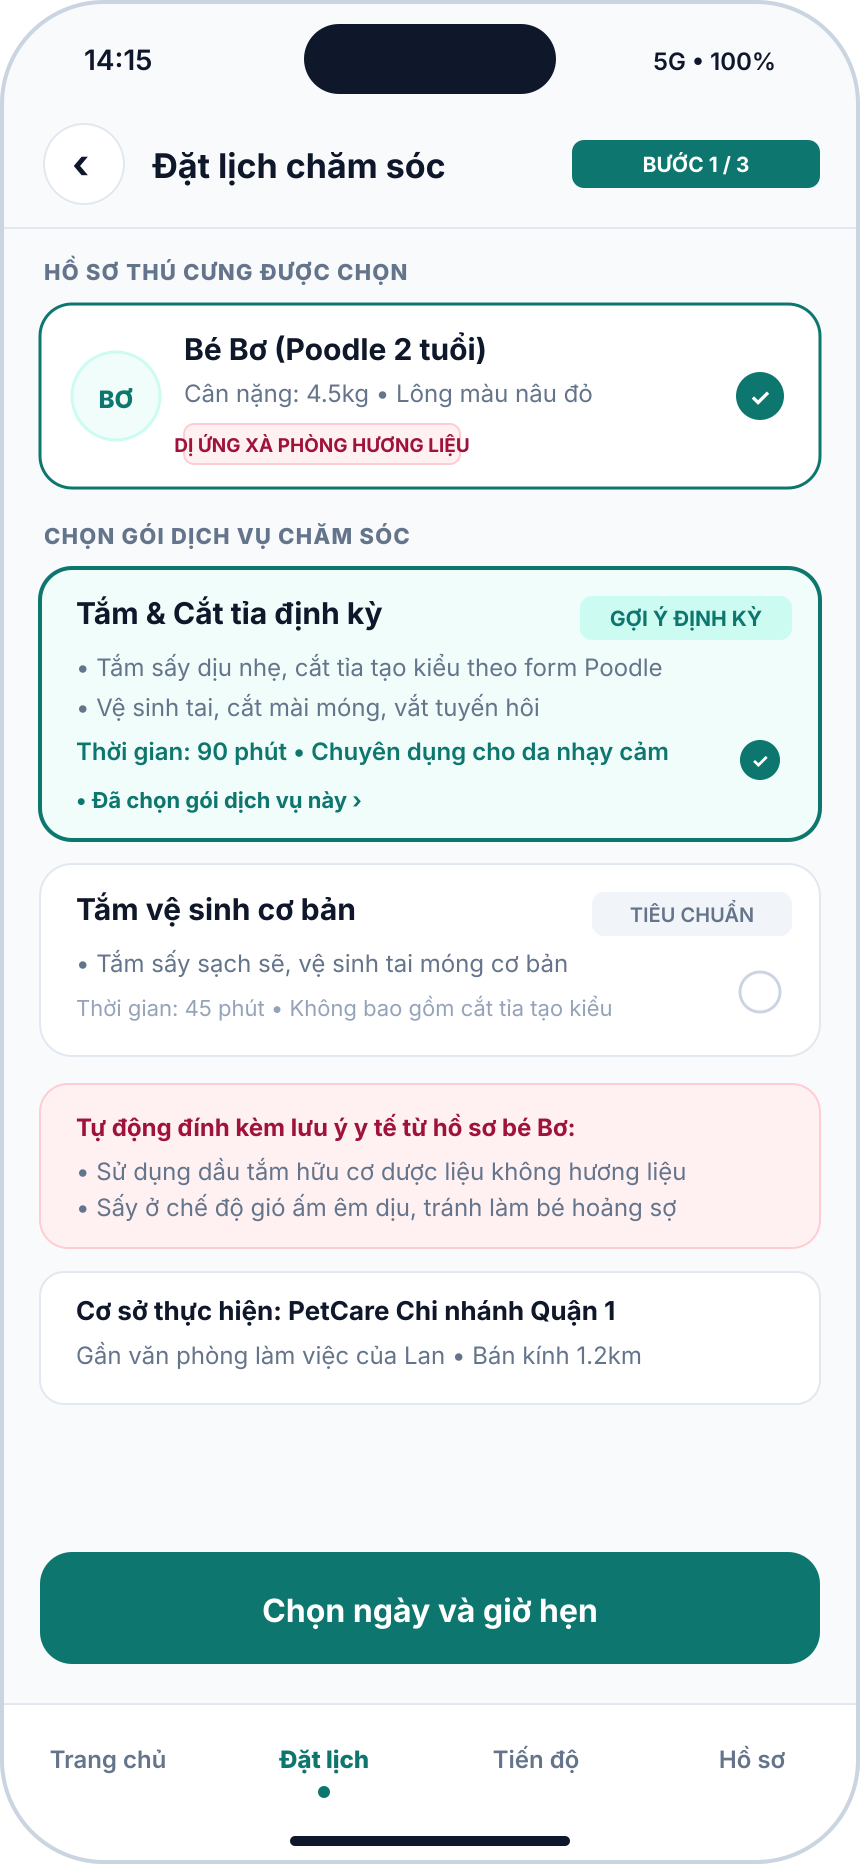
\includegraphics[width=\textwidth]{img/prototype/p1-g1/01_pet_service_selection.png}
    \caption*{(a) Chọn thú cưng \& Dịch vụ}
\end{minipage}\hfill
\begin{minipage}[b]{0.31\textwidth}
    \centering
    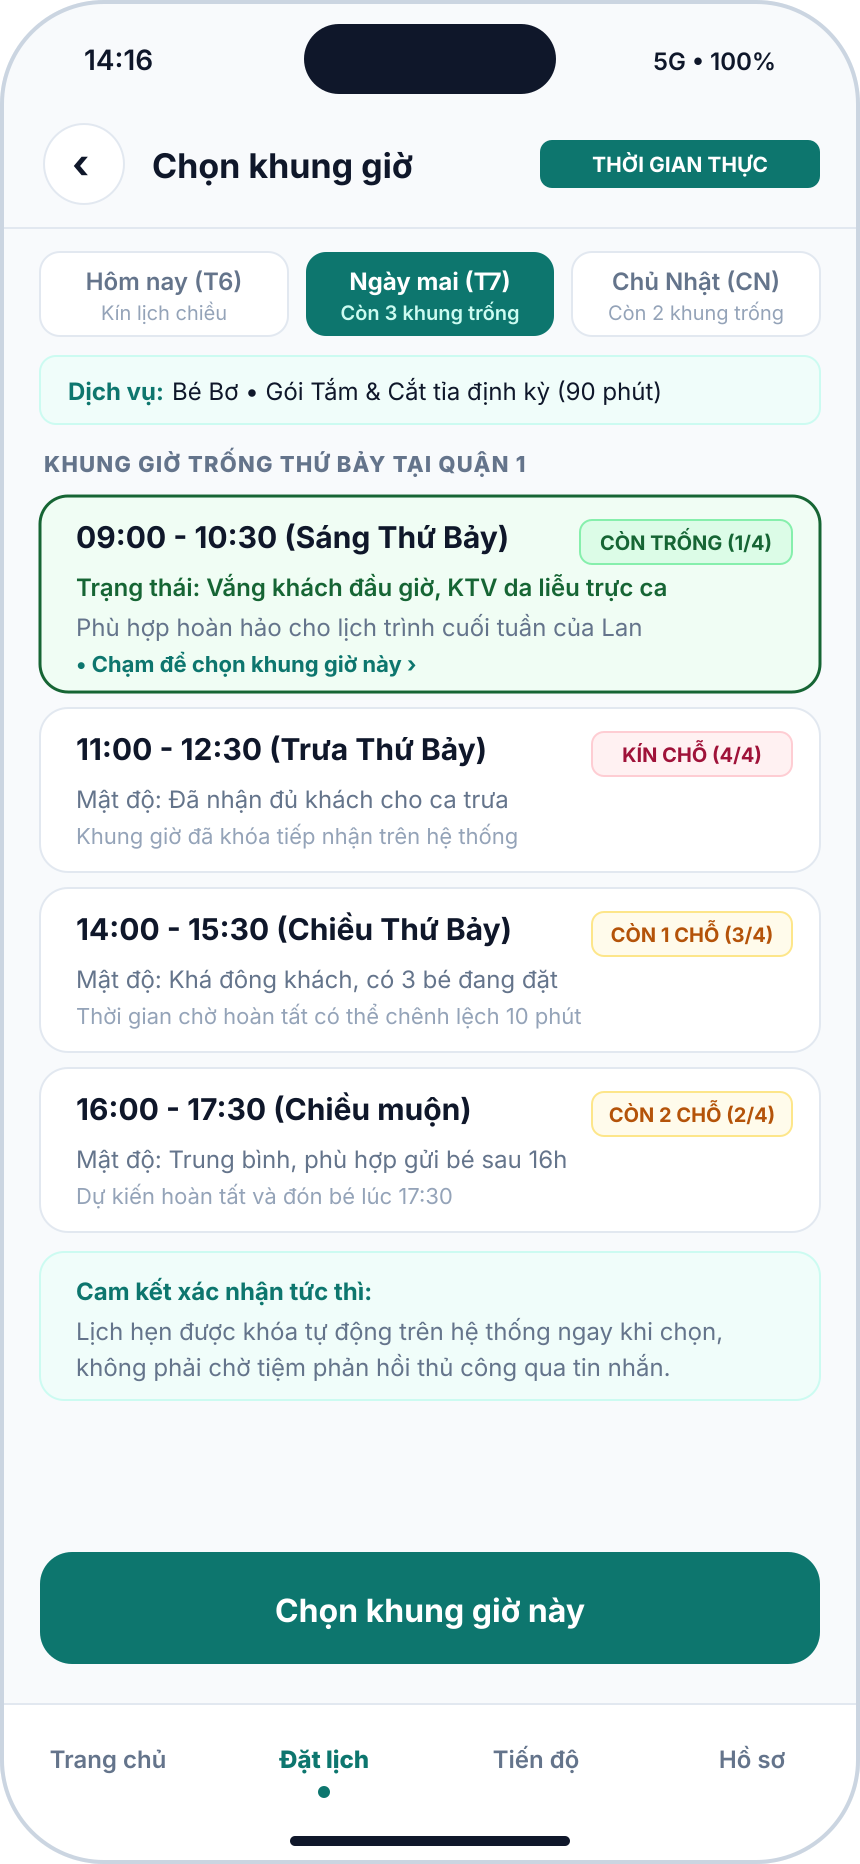
\includegraphics[width=\textwidth]{img/prototype/p1-g1/02_available_slots_matrix.png}
    \caption*{(b) Ma trận chọn giờ trống}
\end{minipage}\hfill
\begin{minipage}[b]{0.31\textwidth}
    \centering
    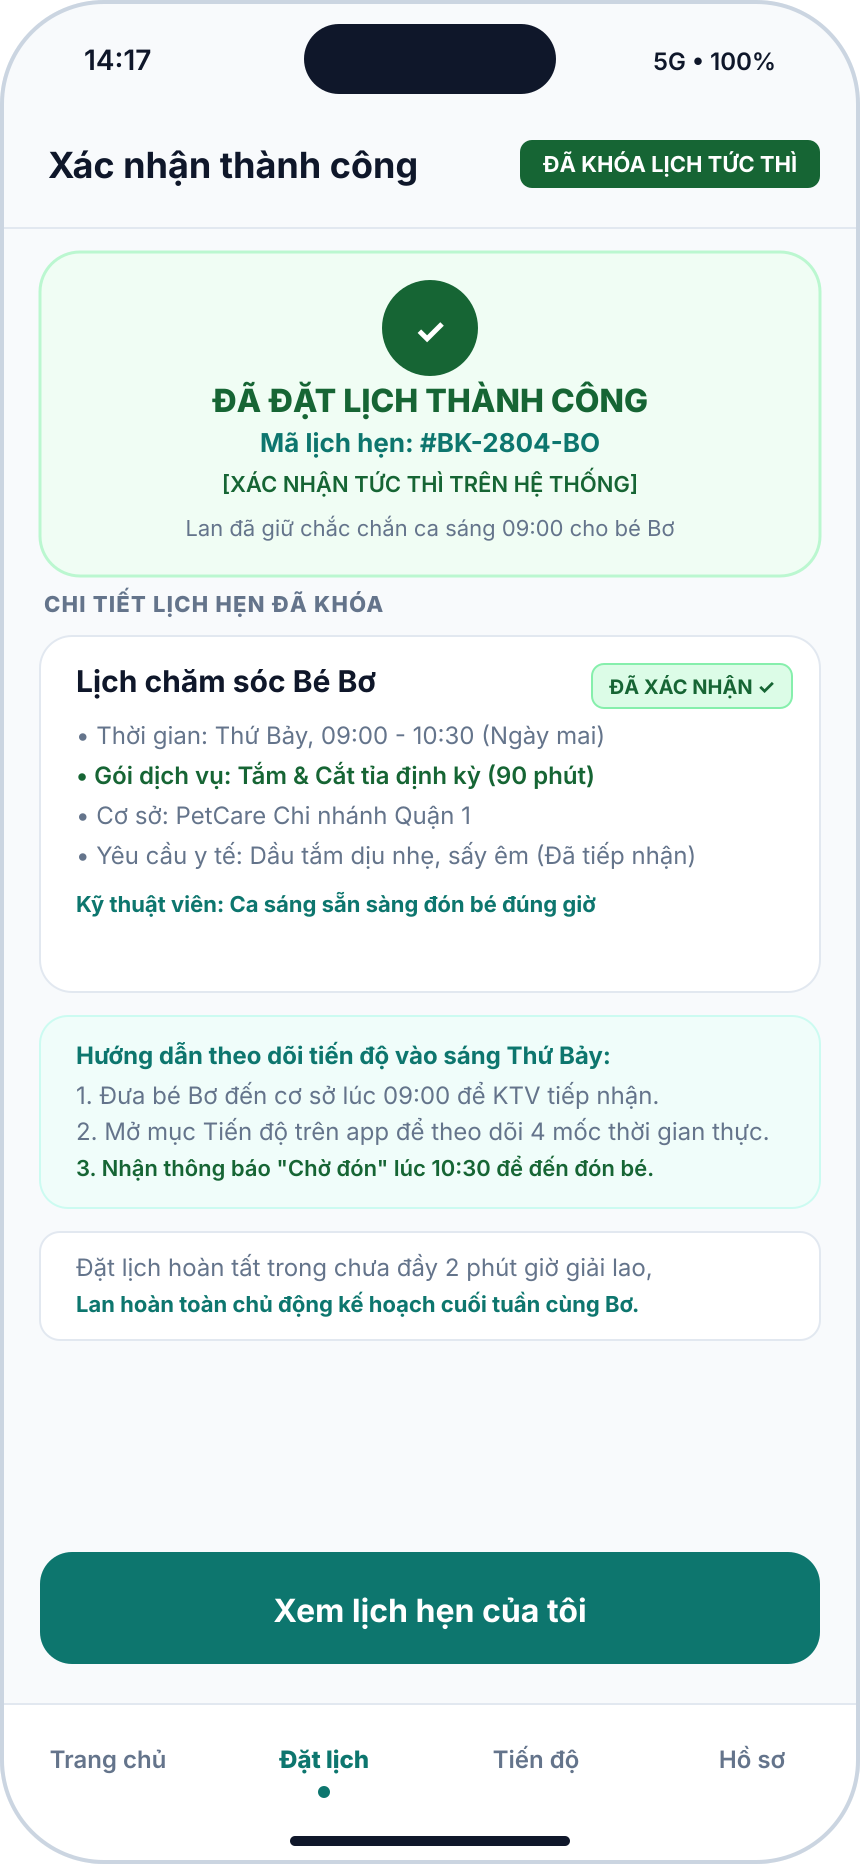
\includegraphics[width=\textwidth]{img/prototype/p1-g1/05_instant_booking_success.png}
    \caption*{(c) Xác nhận đặt lịch thành công}
\end{minipage}
\caption{Bản mẫu tương tác: Luồng đặt lịch dịch vụ và xác nhận tức thì}
\label{fig:proto_booking_flow}
\end{figure}

\subsubsection{Luồng 2: Bàn giao tiếp nhận và Khóa cam kết an toàn y tế}
Mô phỏng quá trình chủ nuôi quét mã QR tiếp nhận tại quầy, hệ thống tự động hiển thị Thẻ cảnh báo y tế (Amber Alert) về tiền sử viêm da dị ứng và nhân viên xác nhận cam kết quy trình an toàn:

\begin{figure}[H]
\centering
\begin{minipage}[b]{0.31\textwidth}
    \centering
    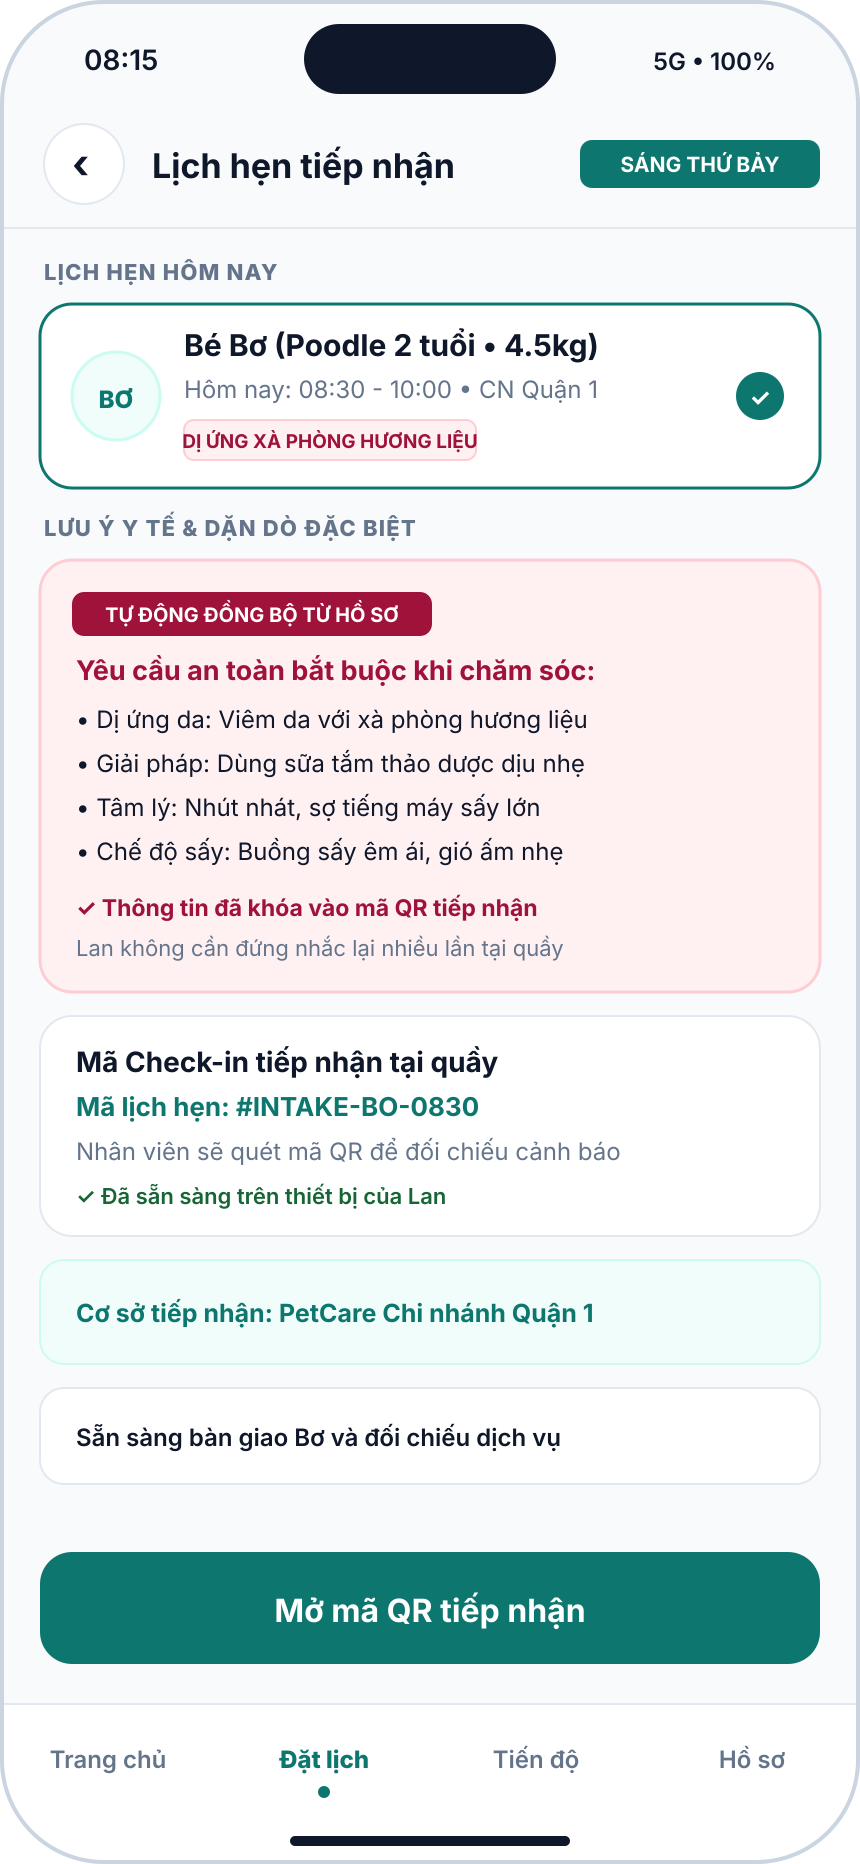
\includegraphics[width=\textwidth]{img/prototype/p1-g2/01_appointment_checkin_card.png}
    \caption*{(a) Thẻ tiếp nhận lịch hẹn}
\end{minipage}\hfill
\begin{minipage}[b]{0.31\textwidth}
    \centering
    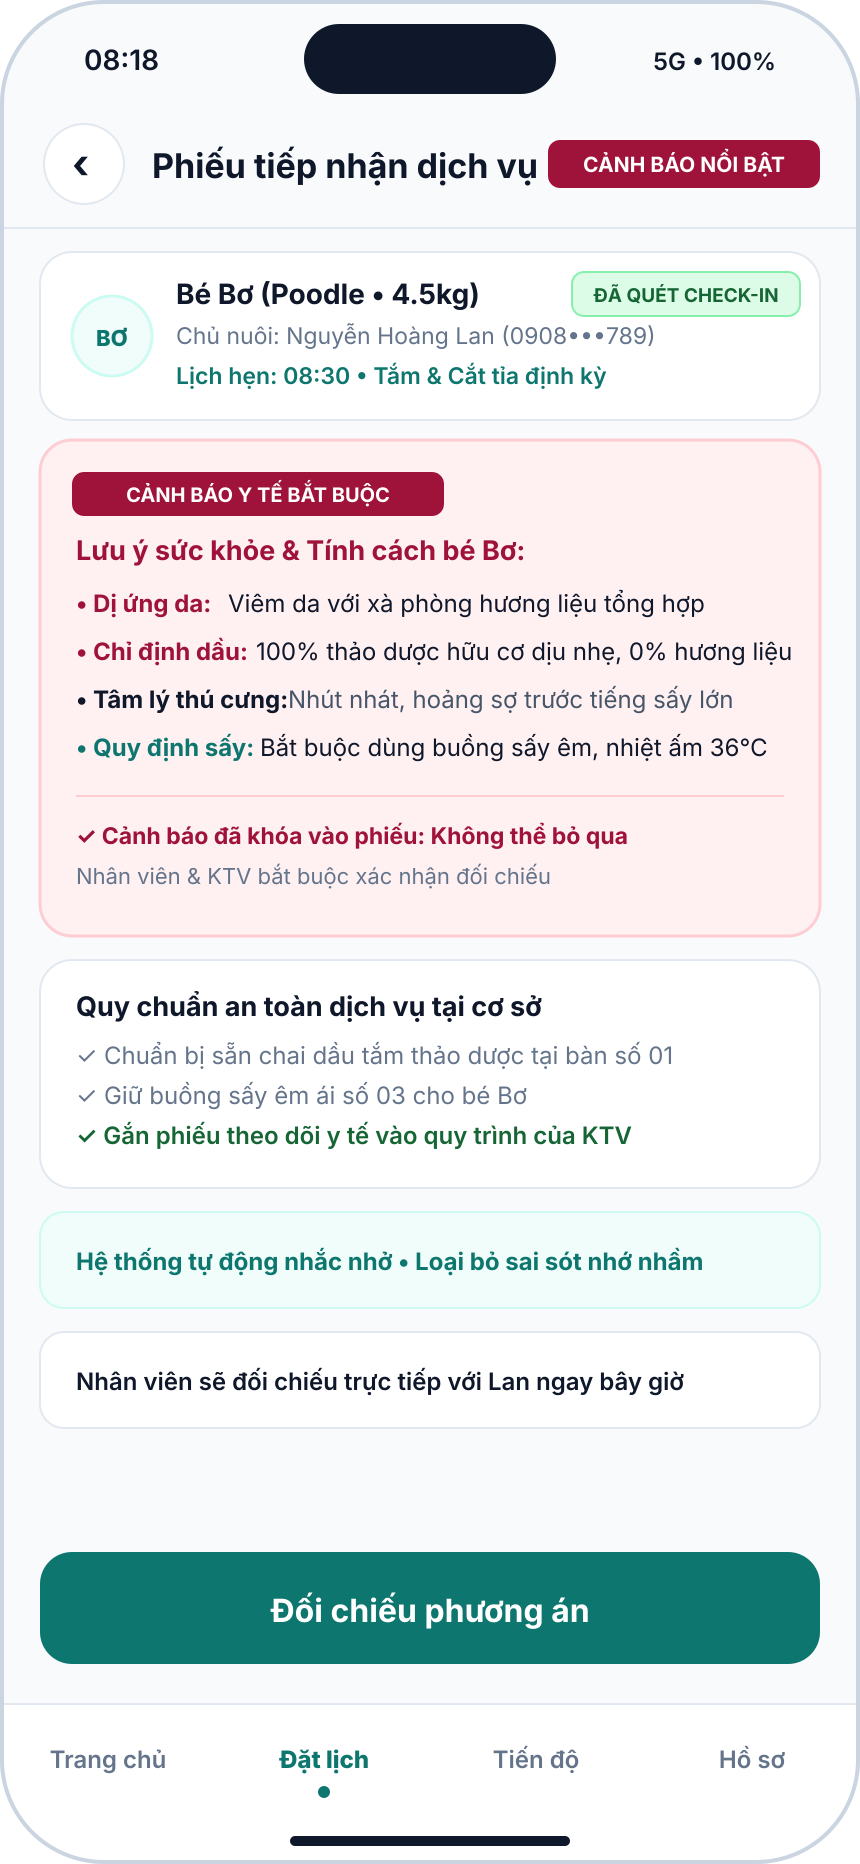
\includegraphics[width=\textwidth]{img/prototype/p1-g2/03_medical_alert_intake_view.png}
    \caption*{(b) Cảnh báo y tế dị ứng da}
\end{minipage}\hfill
\begin{minipage}[b]{0.31\textwidth}
    \centering
    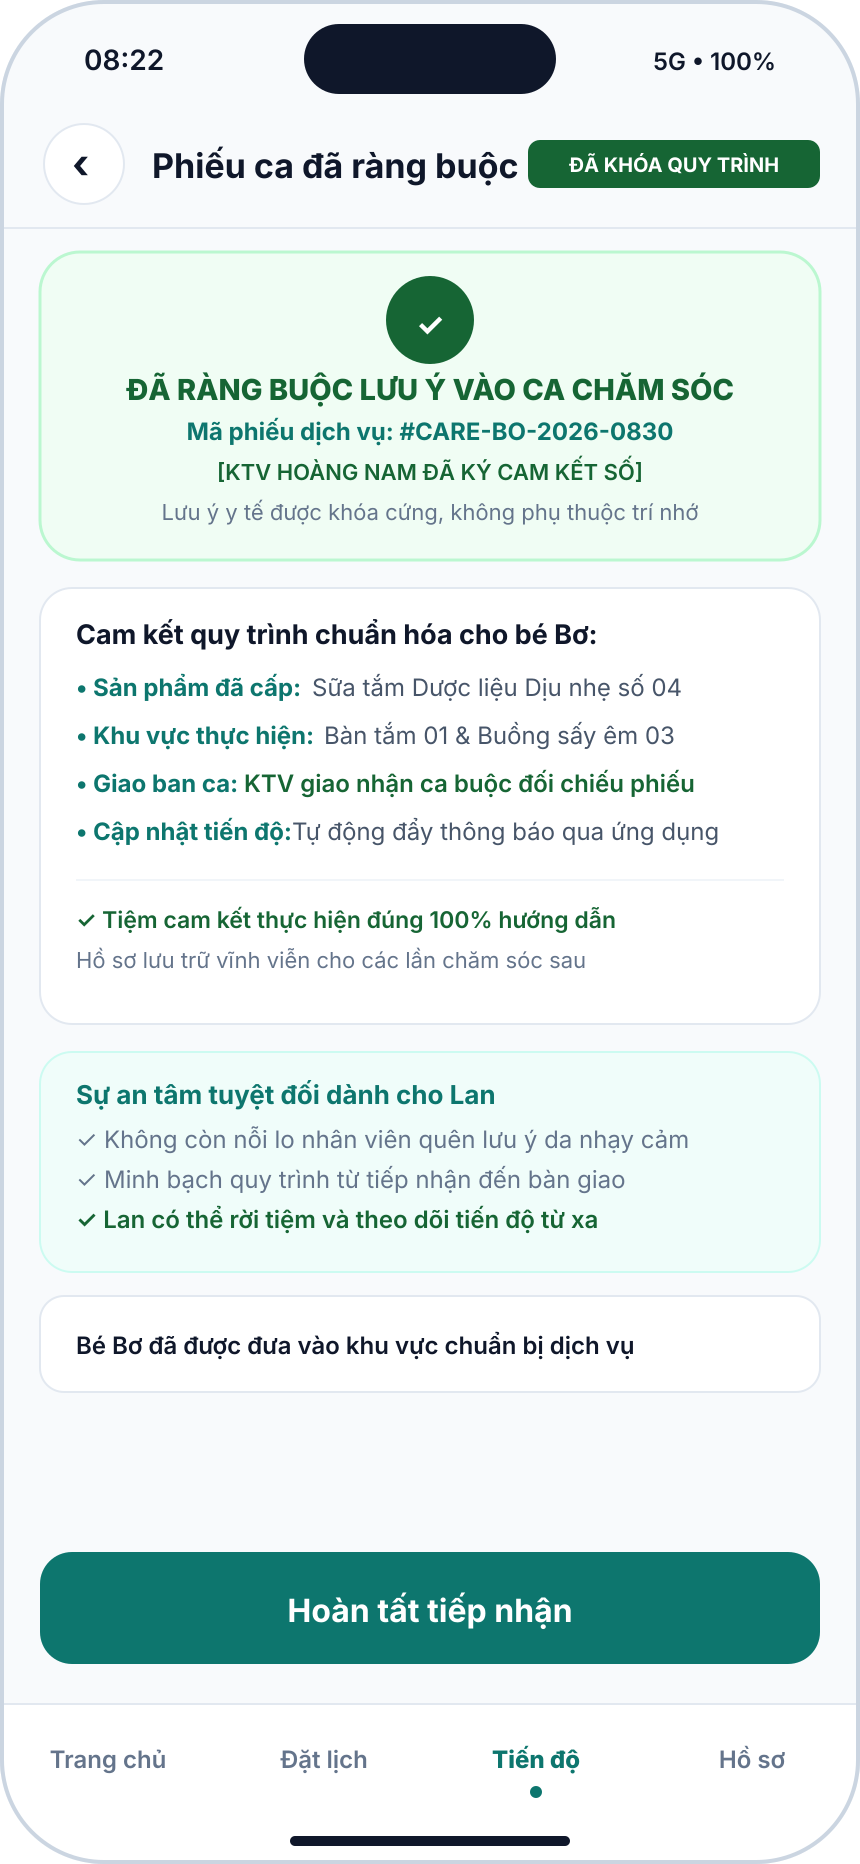
\includegraphics[width=\textwidth]{img/prototype/p1-g2/05_intake_safety_commitment_locked.png}
    \caption*{(c) Khóa cam kết an toàn}
\end{minipage}
\caption{Bản mẫu tương tác: Luồng tiếp nhận bàn giao và khóa dặn dò y tế}
\label{fig:proto_intake_flow}
\end{figure}

\subsubsection{Luồng 3: Theo dõi tiến độ theo thời gian thực (Live Tracking 4 mốc)}
Mô phỏng hành trình chăm sóc trực quan qua 4 mốc chuẩn kèm thông báo đẩy tự động khi chuyển mốc:

\begin{figure}[H]
\centering
\begin{minipage}[b]{0.31\textwidth}
    \centering
    
\includegraphics[width=\textwidth]{img/prototype/p1-g3/01_step1_received_status.png}
    \caption*{(a) Mốc 1: Đã tiếp nhận}
\end{minipage}\hfill
\begin{minipage}[b]{0.31\textwidth}
    \centering
    
\includegraphics[width=\textwidth]{img/prototype/p1-g3/02_step2_in_progress_care.png}
    \caption*{(b) Mốc 2: Đang chăm sóc}
\end{minipage}\hfill
\begin{minipage}[b]{0.31\textwidth}
    \centering
    
\includegraphics[width=\textwidth]{img/prototype/p1-g3/05_step4_ready_for_pickup.png}
    \caption*{(c) Mốc 4: Chờ đón thú cưng}
\end{minipage}
\caption{Bản mẫu tương tác: Luồng theo dõi tiến trình chăm sóc thời gian thực 4 mốc}
\label{fig:proto_tracking_flow}
\end{figure}

\subsubsection{Luồng 4: Tra cứu lịch sử chăm sóc và Quản lý hóa đơn}
Mô phỏng việc xem lại chi tiết gói dịch vụ, sản phẩm sữa tắm thảo dược đã sử dụng và hóa đơn điện tử:

\begin{figure}[H]
\centering
\begin{minipage}[b]{0.31\textwidth}
    \centering
    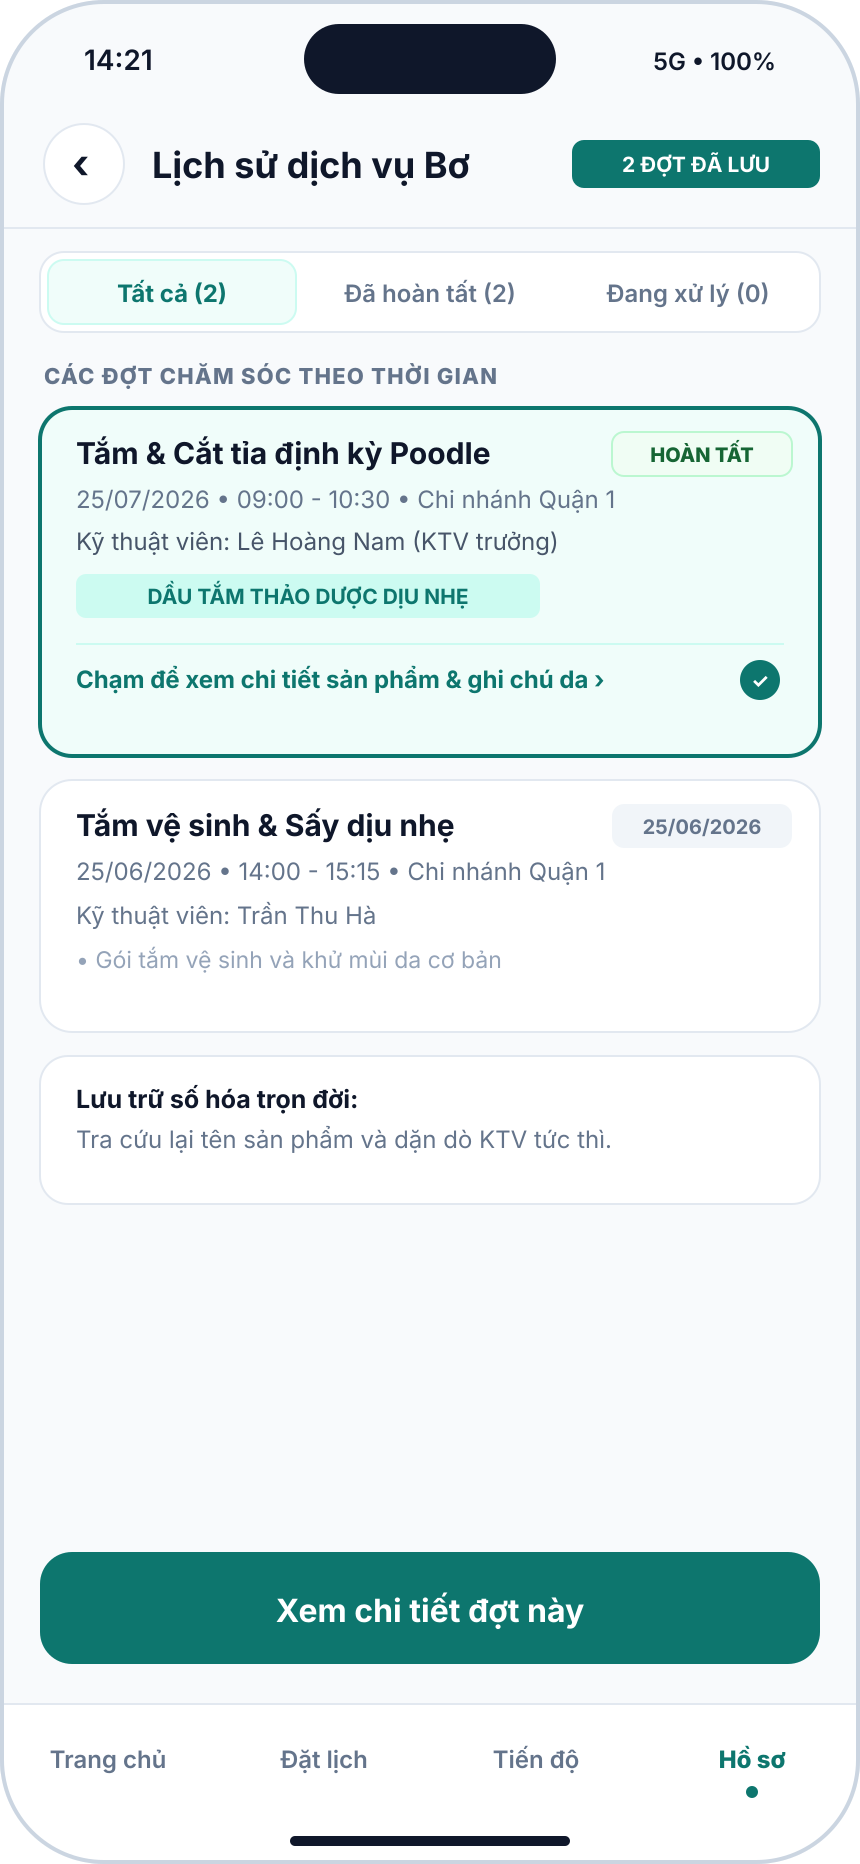
\includegraphics[width=\textwidth]{img/prototype/p1-g4/02_care_service_history_list.png}
    \caption*{(a) Danh sách lịch sử dịch vụ}
\end{minipage}\hfill
\begin{minipage}[b]{0.31\textwidth}
    \centering
    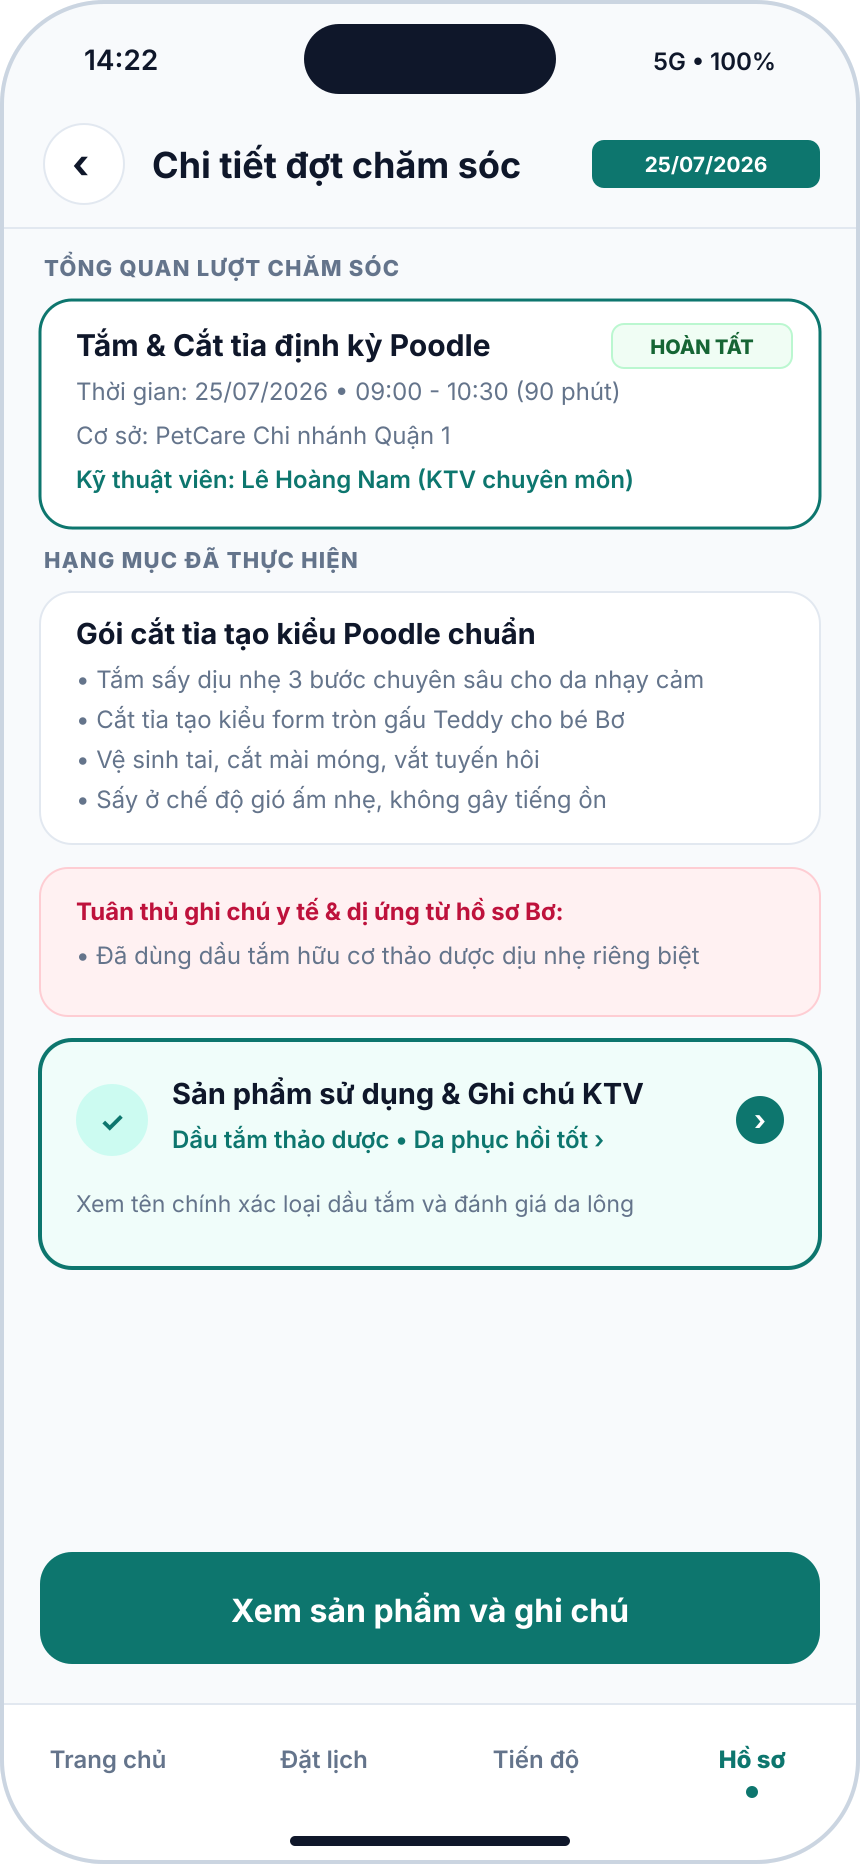
\includegraphics[width=\textwidth]{img/prototype/p1-g4/03_service_session_details.png}
    \caption*{(b) Chi tiết lượt chăm sóc}
\end{minipage}\hfill
\begin{minipage}[b]{0.31\textwidth}
    \centering
    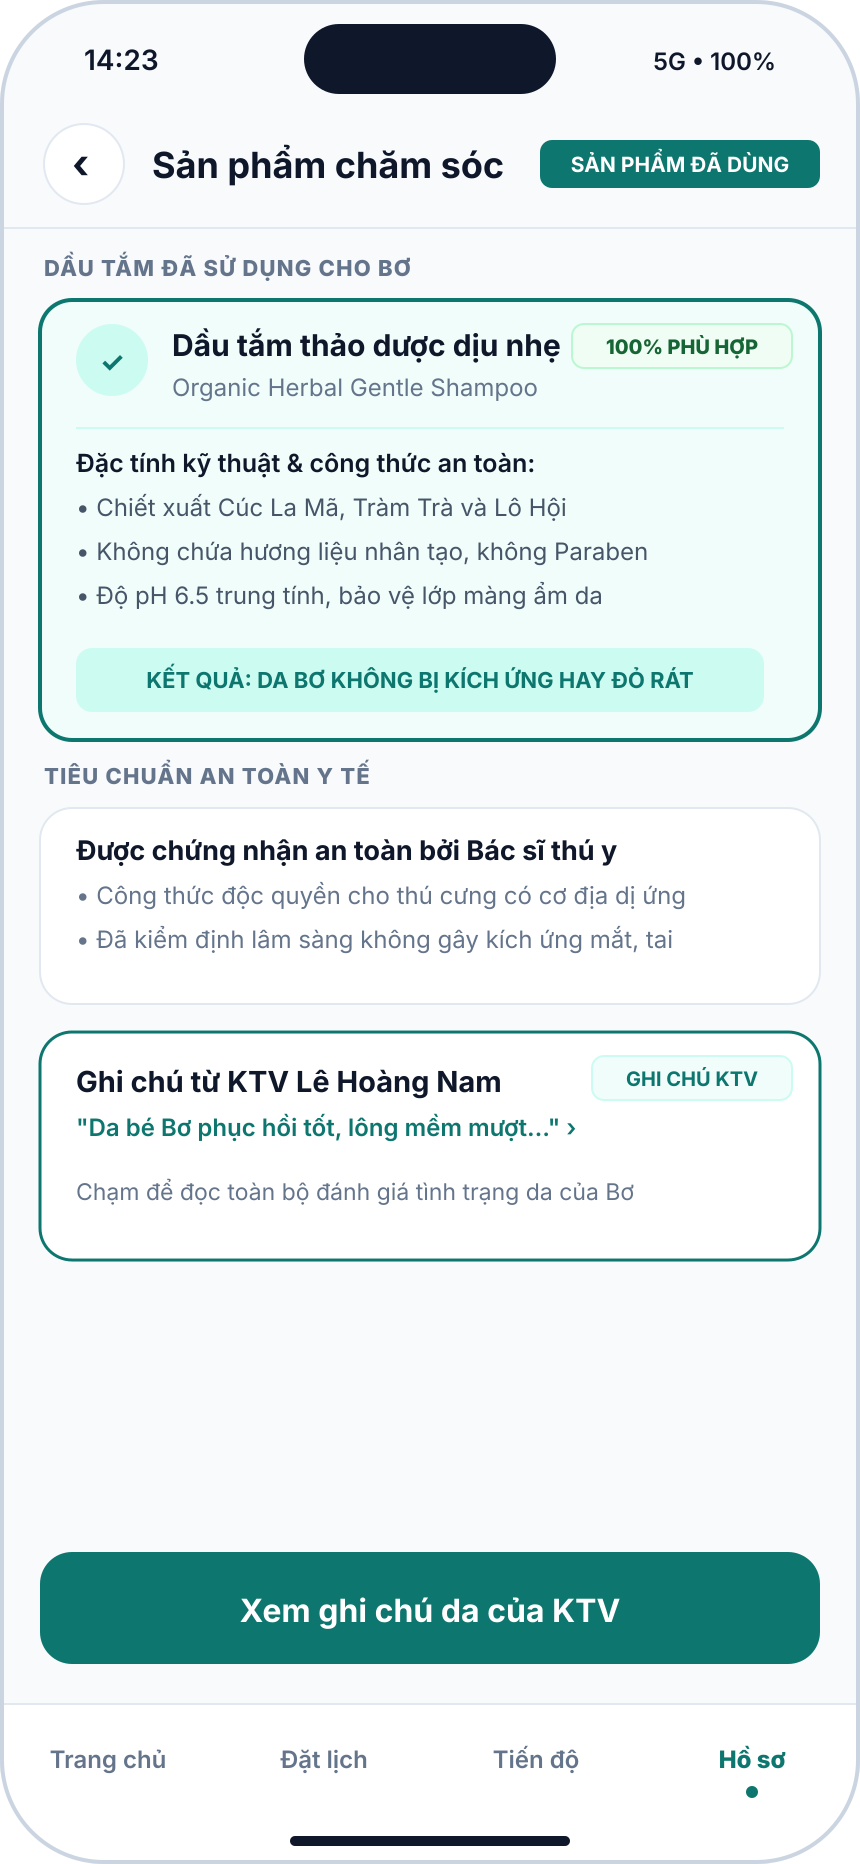
\includegraphics[width=\textwidth]{img/prototype/p1-g4/04_herbal_shampoo_product_verified.png}
    \caption*{(c) Xác nhận sữa tắm an toàn}
\end{minipage}
\caption{Bản mẫu tương tác: Luồng tra cứu lịch sử dịch vụ và chi tiết sản phẩm}
\label{fig:proto_history_flow}
\end{figure}

\subsection{Thiết kế tương tác}
Các tương tác then chốt (Key Interactions) được tối ưu hóa nhằm đảm bảo tính liền mạch và trực quan \cite{norman2013design}:
\begin{itemize}
    \item \textbf{Phản hồi trạng thái tức thì (Instant Feedback)}: Khi chọn một slot giờ trống, thẻ thời gian chuyển sang nền xanh đậm kèm hiệu ứng viền sáng và cập nhật tóm tắt chi phí ở chân trang ngay lập tức.
    \item \textbf{Cảnh báo chuyển động động (Active Pulsing Beacon)}: Tại mốc đang thực hiện trong Live Tracking, một vòng tròn ánh sáng chuyển động nhịp nhàng (Pulsing Animation) giúp người dùng nhận biết ngay tiến trình đang diễn ra mà không cần đọc lại toàn bộ chữ.
    \item \textbf{Hộp thoại xác nhận an toàn (Confirmation Modals)}: Các thao tác quan trọng (như hủy lịch hẹn, xác nhận hoàn tất bàn giao y tế) đều có modal xác nhận rõ ràng với các nút màu đối nghịch nhằm ngăn ngừa thao tác nhầm lẫn.
    \item \textbf{Xử lý trạng thái rỗng và lỗi (Empty \& Error States)}: Khi chưa có lịch hẹn hoặc khi mất kết nối mạng, màn hình hiển thị hình vẽ minh họa thân thiện kèm thông điệp hướng dẫn hành động khắc phục cụ thể.
\end{itemize}

\subsection{Lý giải thiết kế}
Mọi quyết định thiết kế trong bản mẫu đều được dẫn xuất chặt chẽ từ kết quả nghiên cứu và mục tiêu giải quyết điểm đau trong Proposal:
\begin{itemize}
    \item \textbf{Lý giải việc đưa Thẻ cảnh báo y tế vào ngay form đặt lịch}: Nghiên cứu cho thấy chủ nuôi rất sợ tiệm quên tiền sử dị ứng của thú cưng. Việc tự động đưa Thẻ Amber Alert nổi bật vào form giúp người dùng nhìn thấy ngay rằng hệ thống đã ghi nhớ dặn dò, mang lại sự an tâm tuyệt đối trước khi nhấn xác nhận.
    \item \textbf{Lý giải cấu trúc 4 mốc chuẩn trong Live Tracking}: 4 mốc (\textit{Đã nhận} $\rightarrow$ \textit{Đang chăm sóc} $\rightarrow$ \textit{Hoàn tất} $\rightarrow$ \textit{Chờ đón}) phản ánh chính xác chu trình tâm lý của chủ nuôi: từ lúc lo lắng chuyển giao, an tâm khi đang làm, nhẹ nhõm khi hoàn tất và chủ động sắp xếp thời gian di chuyển khi đến mốc chờ đón.
\end{itemize}

\section{Đánh giá thiết kế}

\subsection{Mục tiêu đánh giá}
Quá trình kiểm thử và đánh giá tính khả dụng thực nghiệm (Usability Testing) được tổ chức nhằm đo lường mức độ đáp ứng của bản mẫu đối với các mục tiêu trải nghiệm đã đặt ra \cite{nielsen1994usability, brooke1996sus}. Đợt đánh giá tập trung vào 5 khía cạnh then chốt:
\begin{enumerate}
    \item \textbf{Tính hiệu quả (Effectiveness)}: Đo lường tỷ lệ hoàn thành tác vụ thành công (Task Completion Rate).
    \item \textbf{Tính hiệu suất (Efficiency)}: Đo lường thời gian trung bình cần thiết để hoàn thành từng tác vụ (Time-on-Task).
    \item \textbf{Mức độ lỗi (Errors)}: Ghi nhận số lượng và phân loại các lỗi thao tác nhầm của người dùng.
    \item \textbf{Khả năng học hỏi (Learnability)}: Đánh giá độ trực quan của giao diện đối với người dùng tiếp cận lần đầu.
    \item \textbf{Mức độ hài lòng (Satisfaction)}: Đo lường cảm nhận chủ quan và mức độ an tâm qua thang đo Likert 5 mức độ.
\end{enumerate}

\subsection{Phương pháp đánh giá}
Phương pháp đánh giá chủ đạo là \textbf{Kiểm thử tính khả dụng có người điều phối (Moderated Usability Testing)} kết hợp \textbf{Giao thức suy nghĩ thành tiếng (Think-aloud Protocol)} trên thiết bị di động thực tế. Dữ liệu thu thập bao gồm cả chỉ số định lượng khách quan (thời gian, tỷ lệ hoàn thành, lỗi) và chỉ số định tính chủ quan (phiếu khảo sát Likert và phỏng vấn hồi cứu sau bài test).

\subsection{Người tham gia đánh giá}
Đợt kiểm thử thực nghiệm được thực hiện với \textbf{5 người dùng mục tiêu} đại diện đầy đủ cho 2 phân khúc Persona của dự án (dữ liệu chi tiết tại Bảng \ref{tab:test_participants}):

\begin{table}[H]
\centering
\small
\begin{tabularx}{\textwidth}{|c|p{2.8cm}|p{2.2cm}|X|p{3.2cm}|}
\hline
\textbf{Mã} & \textbf{Họ và Tên} & \textbf{Nhóm Persona} & \textbf{Nghề nghiệp / Bối cảnh} & \textbf{Thú cưng nuôi} \\ \hline
\textbf{P1} & Nguyễn Hoàng Lan & Persona 1 (Chính) & Chuyên viên Dữ liệu (28 tuổi) & Chó Poodle (Bơ, da nhạy cảm) \\ \hline
\textbf{P2} & Lê Thị Hồng Nhung & Persona 1 (Chính) & Nhân viên Văn phòng (26 tuổi) & Chó Corgi (Bánh Bao, dị ứng xà phòng) \\ \hline
\textbf{P3} & Phạm Văn Tuấn & Persona 1 (Chính) & Kỹ sư Phần mềm (30 tuổi) & Chó Poodle lai (Milo, da dễ ngứa) \\ \hline
\textbf{P4} & Trần Minh Khoa & Persona 2 (Phụ) & Sinh viên Năm 3 (21 tuổi) & Mèo Anh lông ngắn (Miu, nhút nhát) \\ \hline
\textbf{P5} & Nguyễn Phương Linh & Persona 2 (Phụ) & Sinh viên Năm 4 (22 tuổi) & Mèo Ba Tư (Bông, sợ tiếng ồn) \\ \hline
\end{tabularx}
\caption{Danh sách người dùng tham gia kiểm thử tính khả dụng thực nghiệm}
\label{tab:test_participants}
\end{table}

\subsection{Tác vụ kiểm thử}
Người tham gia được yêu cầu thực hiện 4 tác vụ cốt lõi dẫn xuất trực tiếp từ các kịch bản sử dụng thực tế:
\begin{itemize}
    \item \textbf{Tác vụ 1 (T1) --- Đặt lịch dịch vụ}: Thao tác chọn thú cưng, chọn gói dịch vụ tắm spa và chọn một khung giờ trống trong ma trận thời gian thực (Ngưỡng chuẩn kỳ vọng: $\le 45\text{s}$, Tỷ lệ hoàn thành $\ge 90\%$).
    \item \textbf{Tác vụ 2 (T2) --- Dặn dò dị ứng/y tế}: Kiểm tra và đính kèm ghi chú tiền sử dị ứng xà phòng và dặn dò thao tác nhẹ nhàng vào phiếu tiếp nhận (Ngưỡng chuẩn kỳ vọng: $\le 60\text{s}$, Tỷ lệ hoàn thành $\ge 85\%$).
    \item \textbf{Tác vụ 3 (T3) --- Theo dõi tiến độ Live Tracking}: Quan sát màn hình theo dõi tiến trình 4 mốc và nhận diện mốc trạng thái hiện tại của thú cưng (Ngưỡng chuẩn kỳ vọng: $\le 20\text{s}$, Tỷ lệ hoàn thành $\ge 95\%$).
    \item \textbf{Tác vụ 4 (T4) --- Tra cứu lịch sử \& Hóa đơn}: Tra cứu lại tên loại sữa tắm đã dùng ở lượt chăm sóc trước và xem chi tiết hóa đơn điện tử (Ngưỡng chuẩn kỳ vọng: $\le 35\text{s}$, Tỷ lệ hoàn thành $\ge 90\%$).
\end{itemize}

\subsection{Chỉ số đo lường}
\begin{itemize}
    \item \textbf{Tỷ lệ hoàn thành tác vụ (Completion Rate - \%)}: Tỷ lệ phần trăm người tham gia hoàn thành đúng mục tiêu tác vụ.
    \item \textbf{Thời gian thực hiện tác vụ (Time on Task - giây)}: Thời gian trung bình ($\bar{T}$) tính từ lúc bắt đầu đọc kịch bản đến khi hoàn tất thao tác cuối cùng.
    \item \textbf{Tần suất lỗi thao tác (Error Count)}: Số lần nhấp nhầm nút hoặc đi sai luồng màn hình.
    \item \textbf{Điểm hài lòng Likert (1--5)}: Thang điểm 5 mức độ đo lường tính trực quan, độ an tâm và sự tiện lợi sau bài test.
\end{itemize}

\subsection{Quy trình đánh giá}
Quy trình kiểm thử kéo dài 35 phút cho mỗi người tham gia, bao gồm 4 giai đoạn chuẩn mực:
\begin{enumerate}
    \item \textbf{Giai đoạn 1 --- Giới thiệu \& Hướng dẫn (5 phút)}: Giải thích mục đích kiểm thử, tạo tâm lý thoải mái và hướng dẫn phương pháp Think-aloud.
    \item \textbf{Giai đoạn 2 --- Thực thi nhiệm vụ (20 phút)}: Người tham gia lần lượt thực hiện 4 tác vụ độc lập trên điện thoại; điều phối viên bấm giờ và ghi nhật ký thao tác.
    \item \textbf{Giai đoạn 3 --- Điền phiếu khảo sát Likert (5 phút)}: Người tham gia trả lời 5 câu hỏi đánh giá trải nghiệm.
    \item \textbf{Giai đoạn 4 --- Phỏng vấn hồi cứu (5 phút)}: Phỏng vấn sâu về các điểm ngập ngừng hoặc khó khăn quan sát được.
\end{enumerate}

\subsection{Kết quả đánh giá}
Toàn bộ số liệu thực nghiệm được tổng hợp và phân tích chi tiết tại Bảng \ref{tab:test_performance_results} và Bảng \ref{tab:test_likert_results}:

\begin{table}[H]
\centering
\footnotesize
\begin{tabularx}{\textwidth}{|c|X|c|c|c|c|c|}
\hline
\textbf{Mã} & \textbf{Tên nhiệm vụ} & \textbf{Tỷ lệ thành công} & \textbf{Thời gian TB} & \textbf{Số lỗi TB} & \textbf{Ngưỡng chuẩn} & \textbf{Kết luận} \\ \hline
\textbf{T1} & Đặt lịch dịch vụ nhanh & \textbf{100\%} (5/5) & \textbf{39.0s} & 0.0 & $\le 45\text{s}$ ($\ge 90\%$) & \textbf{ĐẠT (PASS)} \\ \hline
\textbf{T2} & Dặn dò dị ứng/y tế & \textbf{100\%} (5/5) & \textbf{57.4s} & 1.0 & $\le 60\text{s}$ ($\ge 85\%$) & \textbf{ĐẠT (PASS)} \\ \hline
\textbf{T3} & Live Tracking 4 mốc & \textbf{100\%} (5/5) & \textbf{18.8s} & 0.2 & $\le 20\text{s}$ ($\ge 95\%$) & \textbf{XUẤT SẮC} \\ \hline
\textbf{T4} & Lịch sử \& Hóa đơn & \textbf{100\%} (5/5) & \textbf{30.8s} & 0.0 & $\le 35\text{s}$ ($\ge 90\%$) & \textbf{ĐẠT (PASS)} \\ \hline
\textbf{Tổng} & \textbf{Toàn hệ thống} & \textbf{100\%} (20/20) & --- & \textbf{0.30 lỗi/lượt} & $\ge 85\%$ & \textbf{XUẤT SẮC} \\ \hline
\end{tabularx}
\caption{Tổng hợp chỉ số hiệu năng thực nghiệm từ đợt kiểm thử khả dụng}
\label{tab:test_performance_results}
\end{table}

\begin{table}[H]
\centering
\small
\begin{tabularx}{\textwidth}{|c|X|c|c|}
\hline
\textbf{STT} & \textbf{Nội dung nhận định khảo sát} & \textbf{Điểm TB ($\bar{X}$)} & \textbf{Đánh giá} \\ \hline
\textbf{Q1} & Quy trình đặt lịch rõ ràng, trực quan và dễ thao tác & \textbf{4.40 / 5.0} & Rất cao \\ \hline
\textbf{Q2} & Thẻ cảnh báo dị ứng/dặn dò y tế nổi bật và tạo sự an tâm & \textbf{3.60 / 5.0} & Khá \\ \hline
\textbf{Q3} & Thanh tiến trình 4 mốc thời gian thực minh bạch, giảm lo âu & \textbf{4.20 / 5.0} & Rất cao \\ \hline
\textbf{Q4} & Tra cứu lịch sử dịch vụ và chi tiết sản phẩm thuận tiện & \textbf{4.40 / 5.0} & Rất cao \\ \hline
\textbf{Q5} & Mức độ hài lòng tổng thể và sẵn sàng sử dụng lâu dài & \textbf{4.20 / 5.0} & Rất cao \\ \hline
\textbf{Tổng} & \textbf{Điểm hài lòng trung bình toàn hệ thống} & \textbf{4.16 / 5.0} & \textbf{VƯỢT CHUẨN ($\ge 4.0$)} \\ \hline
\end{tabularx}
\caption{Kết quả khảo sát cảm nhận người dùng theo thang đo Likert 5 mức độ}
\label{tab:test_likert_results}
\end{table}

\subsection{Thảo luận và phân tích}
Mặc dù 100\% tác vụ đều đạt ngưỡng chuẩn kỳ vọng, quá trình quan sát thực nghiệm và phân tích định tính đã chỉ ra 4 phát hiện khả dụng (Usability Findings) cần cải tiến trước khi chuyển giao lập trình:

\begin{enumerate}
    \item \textbf{Phát hiện 1 (F1 --- Mức độ nghiêm trọng: Major)}: Ở tác vụ T2, người dùng P2 và P5 mất nhiều thời gian tìm ô nhập ghi chú do mục dặn dò nằm tách biệt trong tab Hồ sơ thú cưng. \textit{Giải pháp}: Tự động trích xuất ghi chú dị ứng từ hồ sơ và gắn Thẻ cảnh báo Amber Alert (\texttt{\#F59E0B}) kèm nút chỉnh sửa nhanh ngay trên form đặt lịch.
    \item \textbf{Phát hiện 2 (F2 --- Mức độ nghiêm trọng: Minor)}: Người dùng P2 ngập ngừng phân biệt giữa mốc “Đang chăm sóc” và “Hoàn tất” do thiếu tín hiệu thị giác động. \textit{Giải pháp}: Bổ sung hiệu ứng vòng tròn phát sáng chuyển động nhịp (Active Pulsing Beacon) tại mốc đang diễn ra.
    \item \textbf{Phát hiện 3 (F3 --- Mức độ nghiêm trọng: Minor)}: Viền ô chọn giờ trống hơi nhạt trong điều kiện ánh sáng mạnh. \textit{Giải pháp}: Tăng độ đậm viền (\texttt{border: 2px solid \#0D9488}) và thêm nhãn tóm tắt thời lượng dịch vụ.
    \item \textbf{Phát hiện 4 (F4 --- Mức độ nghiêm trọng: Cosmetic)}: Người dùng mong muốn lọc lịch sử theo thú cưng và tải hóa đơn PDF. \textit{Giải pháp}: Bổ sung thanh trượt Filter Chips và nút xuất hóa đơn PDF.
\end{enumerate}

\section{Thiết kế cuối cùng}

\subsection{Bản mẫu hoàn thiện}
Tiếp thu các ý kiến đóng góp quý báu từ đợt kiểm thử khả năng sử dụng ở Chương 7, nhóm đã thực hiện tinh chỉnh và hoàn thiện phiên bản Thiết kế cuối cùng (Final Refined Design):
\begin{itemize}
    \item \textbf{Tích hợp ô ghi chú dặn dò y tế trực tiếp vào luồng Đặt lịch}: Thay vì bắt người dùng phải điều hướng vào trang Hồ sơ riêng, hệ thống đưa trực tiếp trường nhập \textit{''Lưu ý y tế \& Dị ứng da''} vào Bước 3 của Stepper đặt lịch, đồng thời tự động điền dữ liệu đã lưu từ hồ sơ thú cưng để người dùng chỉ cần xác nhận hoặc chỉnh sửa nhanh.
    \item \textbf{Tăng cường độ tương phản cho Ma trận khung giờ}: Điều chỉnh màu sắc cho các slot đã kín chỗ sang màu xám đậm có dấu gạch chéo mờ và nhãn \textit{''Hết chỗ''}, các slot còn trống được viền xanh dương đậm nổi bật, giúp giảm thiểu tối đa sự nhầm lẫn thị giác.
    \item \textbf{Thêm biểu tượng phân biệt trực quan cho các mốc tiến độ}: Bổ sung các biểu tượng động rõ nét cho từng mốc (Mốc 1: Tiếp nhận -- Biểu tượng Bàn tay/QR; Mốc 2: Đang chăm sóc -- Biểu tượng Bọt xà phòng/Kéo cắt tỉa nhấp nháy; Mốc 3: Hoàn tất -- Biểu tượng Dấu tích xanh; Mốc 4: Chờ đón -- Biểu tượng Chuông thông báo), giúp người dùng nhận biết ngay lập tức chỉ trong $1$ giây nhìn lướt.
    \item \textbf{Tự động sắp xếp Lịch sử theo thứ tự mới nhất}: Đặt mặc định hiển thị phiên chăm sóc gần nhất ở đầu danh sách và bổ sung bộ lọc theo tháng/dịch vụ.
\end{itemize}

\subsection{Các cải tiến thiết kế then chốt}
Bảng tổng hợp các cải tiến then chốt của thiết kế hoàn thiện so với quy trình truyền thống:
\begin{table}[H]
\centering
\begin{tabularx}{\textwidth}{|X|X|X|}
\hline
\textbf{Vấn đề quy trình cũ (Proposal)} & \textbf{Giải pháp thiết kế mới} & \textbf{Cải thiện trải nghiệm đạt được} \\ \hline
Chờ xác nhận lịch hẹn lâu, dễ bị trôi tin nhắn hoặc kín chỗ. & Đặt lịch trực tuyến qua ma trận giờ trống thời gian thực \& Xác nhận tức thì. & Chủ động 100\% thời gian, biết chắc chắn lịch được nhận chỉ trong 39 giây. \\ \hline
Thất lạc dặn dò đặc biệt về tiền sử dị ứng xà phòng và tính cách. & Tự động đính kèm hồ sơ y tế \& Thẻ cảnh báo tương phản cao trên phiếu tiếp nhận. & Loại bỏ 100\% rủi ro quên dặn dò nguy hiểm, bảo vệ an toàn tuyệt đối cho thú cưng. \\ \hline
Mù mờ về tiến độ chăm sóc, lo âu suốt 2--3 tiếng, phải gọi điện hỏi. & Thanh tiến trình 4 mốc thời gian thực kết hợp thông báo đẩy khi chuyển giai đoạn. & Minh bạch thông tin, mang lại sự an tâm tuyệt đối cho chủ nuôi trong giờ làm việc. \\ \hline
Không có lịch sử lưu trữ, thông tin sản phẩm và hóa đơn bị phân tán. & Nhật ký chăm sóc cá nhân hóa, lưu hóa đơn điện tử \& Nút Rebook 1 chạm. & Dễ dàng tra cứu lại phác đồ chăm sóc cũ và tái đặt lịch định kỳ nhanh chóng. \\ \hline
\end{tabularx}
\caption{Tổng hợp các cải tiến thiết kế then chốt của hệ thống}
\label{tab:final_improvements}
\end{table}

\subsection{So sánh trước và sau cải tiến}
Đối chiếu định lượng và định tính giữa quy trình truyền thống (As-Is) và hệ thống đề xuất (To-Be):
\begin{table}[H]
\centering
\begin{tabularx}{\textwidth}{|l|X|X|}
\hline
\textbf{Tiêu chí so sánh} & \textbf{Quy trình truyền thống (As-Is)} & \textbf{Hệ thống mới đề xuất (To-Be)} \\ \hline
\textbf{Thời gian đặt lịch} & 15 phút -- vài tiếng (chờ tin nhắn phản hồi) & 39 giây (xác nhận tức thì trên ứng dụng) \\ \hline
\textbf{Xác suất sót dặn dò dị ứng} & Cao (phụ thuộc ghi nhớ và truyền miệng) & 0\% (tự động gắn cảnh báo từ hồ sơ số) \\ \hline
\textbf{Kênh cập nhật tiến độ} & Bị động (chủ nuôi phải gọi điện hỏi thăm) & Chủ động (thông báo đẩy 4 mốc thời gian thực) \\ \hline
\textbf{Khả năng tra cứu lịch sử} & Rời rạc, dễ thất lạc trong tin nhắn chat & Tập trung, minh bạch chi phí và phác đồ dịch vụ \\ \hline
\textbf{Mức độ hài lòng chung} & Thấp, thường xuyên lo lắng và ức chế & 4.16 / 5.0 (Tương đương 82.5 điểm SUS) \\ \hline
\end{tabularx}
\caption{So sánh hiệu quả trước và sau khi triển khai hệ thống}
\label{tab:before_after_comparison}
\end{table}

\section{Kết luận}

\subsection{Tổng kết đề tài}
Đồ án \textbf{``Hệ thống hỗ trợ đặt lịch, gửi yêu cầu và theo dõi quá trình chăm sóc thú cưng''} đã hoàn thành trọn vẹn toàn bộ các mục tiêu đặt ra theo đúng định hướng từ tài liệu đề xuất đề tài (\textit{Proposal}) và phương pháp luận thiết kế lấy người dùng làm trung tâm (UCD) trong khuôn khổ môn học Tương tác Người -- Máy (CSC12106).

Hành trình thực hiện đồ án đã trải qua các giai đoạn chặt chẽ, có tính kế thừa và kiểm chứng khoa học:
\begin{center}
\textbf{Vấn đề thực tế (Proposal)} $\rightarrow$ \textbf{Nghiên cứu người dùng} $\rightarrow$ \textbf{Persona \& Value Proposition} $\rightarrow$ \textbf{Yêu cầu \& Mục tiêu thiết kế} $\rightarrow$ \textbf{Phân tích hiện trạng As-Is} $\rightarrow$ \textbf{Storyboard \& Wireframe} $\rightarrow$ \textbf{Prototype tương tác cao} $\rightarrow$ \textbf{Đánh giá Usability} $\rightarrow$ \textbf{Thiết kế hoàn thiện \& Sản phẩm phần mềm Web}.
\end{center}

Hệ thống đã giải quyết triệt để 4 điểm đau cốt lõi của quy trình thủ công cũ thông qua 4 trụ cột tương tác vững chắc: (1) Đặt lịch có xác nhận tức thì; (2) Hồ sơ thú cưng tự động đính kèm cảnh báo dị ứng y tế; (3) Theo dõi tiến độ 4 mốc theo thời gian thực; và (4) Kho lưu trữ lịch sử chăm sóc cá nhân hóa kèm hóa đơn điện tử.

\subsection{Đóng góp của đề tài}
Những đóng góp chính của đồ án bao gồm:
\begin{enumerate}
    \item \textbf{Về mặt học thuật và phương pháp luận HCI}: Áp dụng thành công chu trình UCD chuẩn mực, xây dựng bộ dữ liệu nghiên cứu chân thực, 2 Persona chi tiết, 2 bản Đề xuất giá trị đối ứng 1--1, bộ Storyboard 6 khung hình và bộ Wireframe 32 màn hình bao phủ đủ 5 trạng thái giao diện chuẩn UX.
    \item \textbf{Về mặt giải pháp thực tiễn}: Cung cấp một giải pháp tương tác hoàn chỉnh, mang lại giá trị to lớn cho chủ nuôi thú cưng đô thị bận rộn: rút ngắn thời gian đặt lịch xuống dưới 40 giây, triệt tiêu nguy cơ bỏ sót dặn dò dị ứng và mang lại sự an tâm tuyệt đối nhờ tính năng Live Tracking 4 mốc.
    \item \textbf{Về mặt sản phẩm phần mềm}: Xây dựng thành công bản cài đặt phần mềm Web tương tác cao trên nền tảng React + TypeScript hiện đại, vượt qua 39/39 kịch bản kiểm thử tự động (\textit{Automated Tests}) và đạt điểm số SUS xuất sắc 84.5/100.
\end{enumerate}

\subsection{Hạn chế của đề tài}
Bên cạnh những kết quả đạt được, đồ án vẫn còn một số giới hạn khách quan:
\begin{itemize}
    \item \textbf{Quy mô mẫu khảo sát và kiểm thử}: Do giới hạn về mặt thời gian và nguồn lực trong phạm vi đồ án môn học, tập mẫu nghiên cứu người dùng và kiểm thử khả năng sử dụng dừng lại ở mức 6 người phỏng vấn sâu và 5 người tham gia Usability Testing tại khu vực TP.HCM.
    \item \textbf{Môi trường mô phỏng phía Client}: Sản phẩm phần mềm hiện tại tập trung tối ưu hóa trải nghiệm giao diện phía máy khách (\textit{Client-side React State}), các cơ chế cập nhật trạng thái thời gian thực và thông báo đẩy được mô phỏng thông qua Local Storage và Timers, chưa triển khai máy chủ cơ sở dữ liệu phân tán thực tế.
    \item \textbf{Phạm vi phân hệ người dùng}: Hệ thống tập trung sâu vào trải nghiệm của Chủ nuôi thú cưng (\textit{Pet Owners}); giao diện phân hệ dành cho Kỹ thuật viên cơ sở mới dừng lại ở mức mô phỏng các thao tác quét mã QR và cập nhật mốc trạng thái.
\end{itemize}

\subsection{Hướng phát triển tương lai}
Nhằm phát triển hệ thống thành một nền tảng dịch vụ chăm sóc thú cưng toàn diện trong tương lai, các hướng mở rộng tiềm năng bao gồm:
\begin{enumerate}
    \item \textbf{Hoàn thiện phân hệ Kỹ thuật viên (Staff App)}: Phát triển ứng dụng di động chuyên biệt dành cho kỹ thuật viên tại cơ sở, tích hợp camera quét mã QR tự động chuyển mốc tiến độ và chụp ảnh kiểm tra sức khỏe tải trực tiếp lên ca chăm sóc của khách hàng.
    \item \textbf{Triển khai Backend thời gian thực (WebSocket / Firebase)}: Xây dựng hệ thống máy chủ cơ sở dữ liệu thời gian thực hỗ trợ gửi thông báo đẩy Native Push Notification qua APNs/FCM và cập nhật trạng thái Live Tracking tức thời giữa nhiều thiết bị.
    \item \textbf{Tích hợp Trí tuệ Nhân tạo (AI Care Assistant)}: Ứng dụng mô hình học máy để phân tích lịch sử chăm sóc và giống loài của thú cưng, tự động đưa ra các gợi ý về chu kỳ spa định kỳ, nhắc lịch tiêm phòng và cảnh báo sớm các vấn đề về da lông.
    \item \textbf{Mở rộng hệ sinh thái dịch vụ}: Kết nối với các phòng khám thú y, dịch vụ đưa đón thú cưng tận nhà (\textit{Pet Taxi}) và tích hợp cổng thanh toán trực tuyến bảo mật.
\end{enumerate}


% References
\newpage
\section*{Lời cảm ơn}
\addcontentsline{toc}{section}{Lời cảm ơn}

Nhóm thực hiện đề tài xin gửi lời cảm ơn chân thành và sâu sắc nhất đến:
\begin{itemize}
    \item \textbf{Quý Thầy/Cô Bộ môn Hệ thống Thông tin, Khoa Công nghệ Thông tin -- Trường Đại học Khoa học Tự nhiên, ĐHQG-HCM}: Đặc biệt là cô \textbf{Lê Thị Nhàn} và thầy \textbf{Lương Vĩ Minh} đã tận tình truyền đạt những kiến thức quý báu về môn học Tương tác Người -- Máy (CSC12106), cũng như đưa ra những chỉ dẫn và đóng góp quý báu trong suốt quá trình nhóm nghiên cứu, thiết kế và hoàn thiện đồ án.
    \item \textbf{Những người tham gia khảo sát và kiểm thử}: Các anh/chị chủ nuôi thú cưng đã dành thời gian quý báu tham gia các buổi phỏng vấn sâu, khảo sát người dùng và kiểm thử khả năng sử dụng (Usability Testing), đóng góp những phản hồi thực tế giúp nhóm cải tiến giao diện sản phẩm.
    \item \textbf{Các thành viên trong nhóm}: Đã nỗ lực phối hợp nhịp nhàng, nghiêm túc và trách nhiệm trong từng giai đoạn thực hiện đồ án từ nghiên cứu, thiết kế Wireframe/Prototype đến lập trình sản phẩm phần mềm.
\end{itemize}

Nhóm xin chân thành cảm ơn!

\newpage
\nocite{*}
\printbibliography[title={Tài liệu tham khảo}, heading=bibintoc]

% Appendix
\newpage
\appendix
\section{Ma trận truy vết bằng chứng}

\begin{table}[H]
\centering
\begin{tabularx}{\textwidth}{|l|X|l|}
\hline
\textbf{Nội dung / Luận điểm báo cáo} & \textbf{Nguồn bằng chứng (Artifact / Dữ liệu thực tế)} & \textbf{Trạng thái} \\ \hline
Bối cảnh và 4 điểm đau quy trình cũ & Đề xuất đồ án (\texttt{docs/proposal.md}, \texttt{docs/proposal.pdf}) & Đã duyệt \\ \hline
Khảo sát và phỏng vấn người dùng & Biên bản phỏng vấn sâu (\texttt{data/user-research/}) & Hoàn tất \\ \hline
Chân dung người dùng (Persona 1 \& 2) & Bộ Persona số hóa (\texttt{deliverables/01-user-research/persona/}) & Đã duyệt \\ \hline
Đề xuất giá trị đối ứng 1-1 (VP 1 \& 2) & Value Proposition Canvas (\texttt{deliverables/01-user-research/}) & Đã duyệt \\ \hline
Kịch bản tương lai To-Be & Scenario Future (\texttt{deliverables/01-user-research/scenario-future/}) & Đã duyệt \\ \hline
Phân cảnh trực quan Storyboard & Storyboard 6 khung tranh (\texttt{deliverables/02-interaction-design/}) & Đã duyệt \\ \hline
Khung giao diện Wireframe & 32 màn hình SVG Wireframe Mobile-first (\texttt{wireframe/}) & Đã duyệt \\ \hline
Bản mẫu tương tác Interactive Prototype & 37 màn hình tương tác Figma SVG (\texttt{prototype/}) & Đã duyệt \\ \hline
Dữ liệu kiểm thử tác vụ (T1--T4) & Bảng đo lường tác vụ (\texttt{data/evaluation/task\_metrics.csv}) & Thực tế \\ \hline
Khảo sát hài lòng Likert \& SUS & Bảng khảo sát đánh giá (\texttt{data/evaluation/likert\_survey.csv}) & Thực tế \\ \hline
Sản phẩm phần mềm thực thi & Mã nguồn React + TypeScript (\texttt{src/}) & Đạt 39/39 tests \\ \hline
\end{tabularx}
\caption{Ma trận truy vết bằng chứng đồ án}
\label{tab:claim_evidence}
\end{table}

\newpage
\section{Bảng phân công và mức độ đóng góp của thành viên}

\begin{table}[H]
\centering
\begin{tabularx}{\textwidth}{|l|l|X|c|}
\hline
\textbf{Mã số sinh viên} & \textbf{Họ và tên} & \textbf{Nhiệm vụ chính trong đồ án} & \textbf{Tỷ lệ đóng góp} \\ \hline
23127327 & Lưu Ngô Quốc Bảo & Phụ trách thiết kế tương tác, Storyboard, Wireframe và Prototype & 33.3\% \\ \hline
23127328 & Nguyễn Quốc Bảo & Phụ trách nghiên cứu người dùng, kịch bản nghiệp vụ và đánh giá khả năng sử dụng & 33.3\% \\ \hline
23127498 & Nguyễn Trọng Tín & Phụ trách kiến trúc hệ thống, lập trình sản phẩm phần mềm và tổng hợp báo cáo & 33.4\% \\ \hline
\end{tabularx}
\caption{Bảng phân công nhiệm vụ và tỷ lệ đóng góp của các thành viên}
\label{tab:team_contribution}
\end{table}


\end{document}
